\hypertarget{sec:introduction}{%
\section{Introduction}\label{sec:introduction}}

Climate change is one of the most pressing issues globally, and demands
action today. Organisations increasingly focus on sustainable
initiatives, which contribute to transforming societies towards
sustainability (\protect\hyperlink{ref-bradbury1999}{Bradbury \& Clair,
1999}).

Chainge is an organisation contributing to this transformation. Chainge
was established in 2019 by Paul Blakemore and Torben Damgaard Nielsen
who promote sustainable goods transportation. The ambition for Chainge
is to reduce the number of diesel vans transporting goods in Copenhagen
by offering a sustainable alternative that reduces particle pollution
and CO\textsubscript{2} emissions. Chainge does this by utilising
electric cargo bikes to deliver packages from Business-to-Business and
Business-to-Consumers
(\protect\hyperlink{ref-chaingeA2021}{{``Chainge,''} 2021a}).

Chainge's mission aligns with FN's Sustainability Goals, more
specifically number 11
(\protect\hyperlink{ref-chaingeB2021}{{``Chainge,''} 2021b}) and number
13. Goal number 11 entails promoting sustainable cities and communities
(\protect\hyperlink{ref-un2021sustainable}{United Nations, 2021}), while
goal number 13 entails curbing climate chainge by reducing greenhouse
gas emissions. Sustainability is thus deeply embedded within Chainge's
business model and strategy sec.~\ref{sec:conclusion}.

\hypertarget{sec:case_description}{%
\subsection{Case description}\label{sec:case_description}}

One of the primary concerns of Chainge is to increase their drop-off
rate for the new bike drivers. Every minute during delivery has an
impact on the profitability of Chainge's business model and cost for its
customers. In this regard, it is vital that new drivers are onboarded as
efficiently as possible. The overall goal of this project is therefore
to optimise the drop-off rate of deliveries by focusing on optimising
the onboarding process.

The scope of the project is to improve the onboarding process for new
Drivers, as the bike drivers are called. The current process was
presented by the Founder and CEO of the company, Torben, and was
described as an unstructured process that could be improved.
Nonetheless, the flow of the process and the sequence of actions seemed
to be working well. Therefore, our focus is not to redesign the entire
process but to explore what and how information should be delivered to
the new employees at the beginning of their employment.

Furthermore, we decided on this topic because we identified an
opportunity for combining our competencies to accomodate Chainge's need
for reducing the drop-off rate in combination with onboarding new
Drivers.

\hypertarget{sec:research_statement}{%
\subsection{Research statement}\label{sec:research_statement}}

The identified problem is ineffective communication between the
management and the Drivers at Chainge. It results in an unstructured
onboarding process.

\begin{itemize}
\tightlist
\item
  \emph{Research question 1}: What challenges affect the Drivers in the
  onboarding process at Chainge?
\item
  \emph{Research question 2}: How might we improve the onboarding
  process to make it more efficient for the Drivers and Chainge?
\end{itemize}

\hypertarget{sec:methods}{%
\section{Methods}\label{sec:methods}}

Addressing the research questions required gaining insights into Chainge
as an organisation and collective of workers. These insights were
obtained through a qualitative assessment of the work culture and
employees' responsibilities, by conducting three interviews with newly
hired (less than four weeks in their position) Drivers, and then
analysing the collected data.

\textbf{START double diamond}

This process was structured through the Double Diamond model, as it is
described by Norman, D (\protect\hyperlink{ref-norman2002design}{2002}),
fig.~\ref{fig:norman_double_diamond}. We planned the phases of our
inquiry into the problem area, and the development of our solution, and
used the model as a guiding reference point throughout the process. As
our approach was neither agile nor iterative, the final documented
process ended up fitting well onto the Double Diamond model, as we
diverged into the problem area, converged on a specific problem,
diverged into the solutions, and converged on developing a prototype,
fig.~\ref{fig:double_diamond}.

\begin{figure}
\hypertarget{fig:norman_double_diamond}{%
\centering
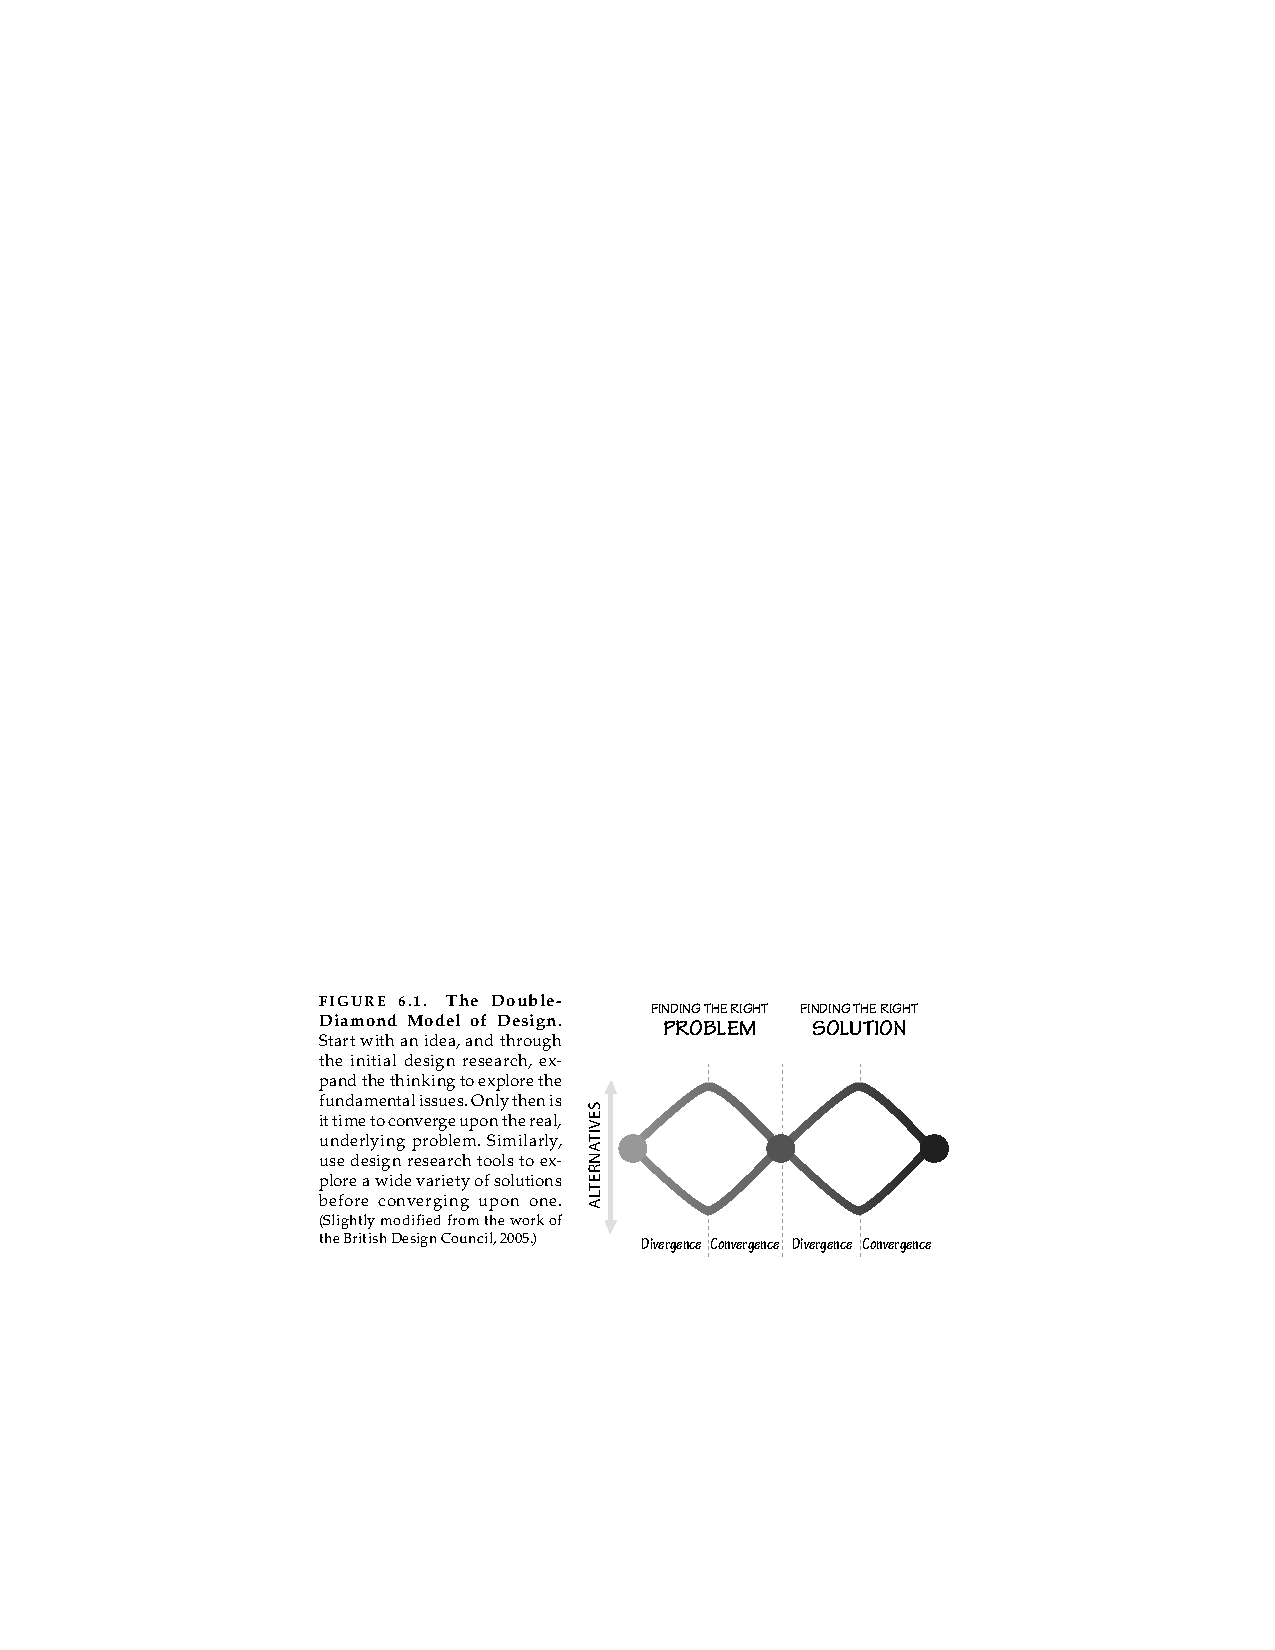
\includegraphics[width=1\textwidth,height=\textheight]{./figures/norman_double_diamond.pdf}
\caption{This is caption}\label{fig:norman_double_diamond}
}
\end{figure}

\begin{figure}
\hypertarget{fig:double_diamond}{%
\centering
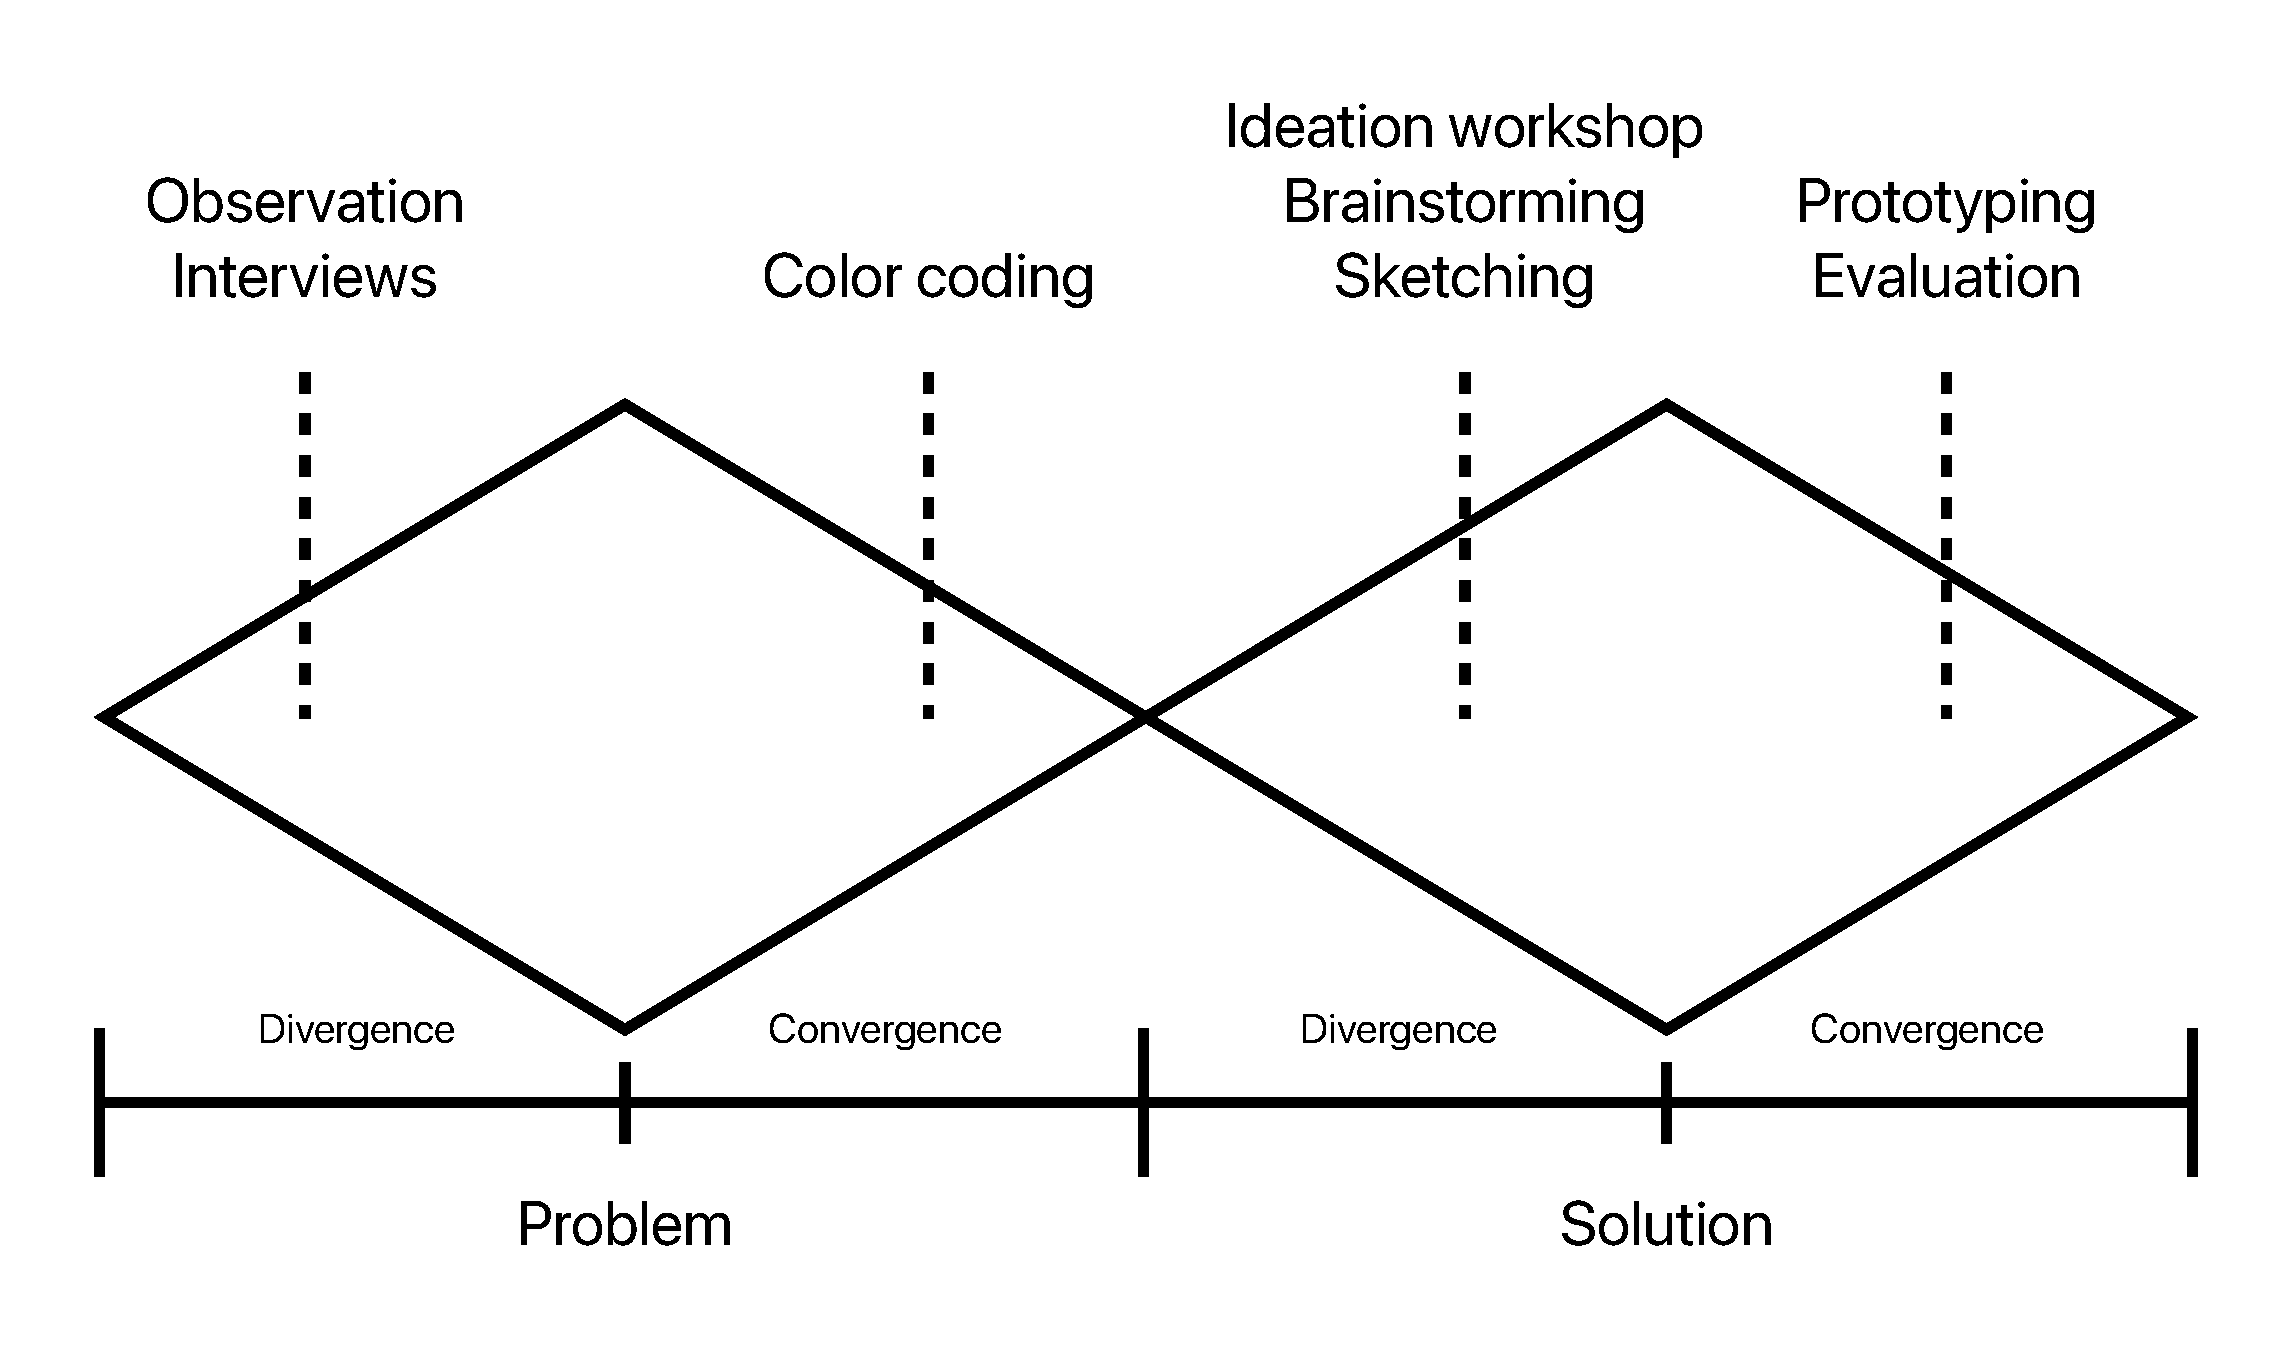
\includegraphics[width=1\textwidth,height=\textheight]{./figures/double_diamond.pdf}
\caption{This is caption}\label{fig:double_diamond}
}
\end{figure}

\textbf{END double diamond}

\hypertarget{sec:interviews}{%
\subsection{Interviews}\label{sec:interviews}}

As part of the empirical gathering, we interviewed Torben, the Founder
and CEO of Chainge, to get an understanding of the business in general
and the onboarding process. The interview was informal and involved an
introduction to the facilities at the headquarters and the electric
cargo bikes. Due to the nature of the interview, we had not created an
interview guide. The interview was informative and provided a great
understanding of the business and strategy. The session with Torben also
had a positive impact on our collaboration due to the informal talk in
between case related subjects. Nevertheless, the interview supported us
in clarifying and guiding us towards the next step in the process.

\begin{pandoccrossrefsubfigures}

\subfloat[]{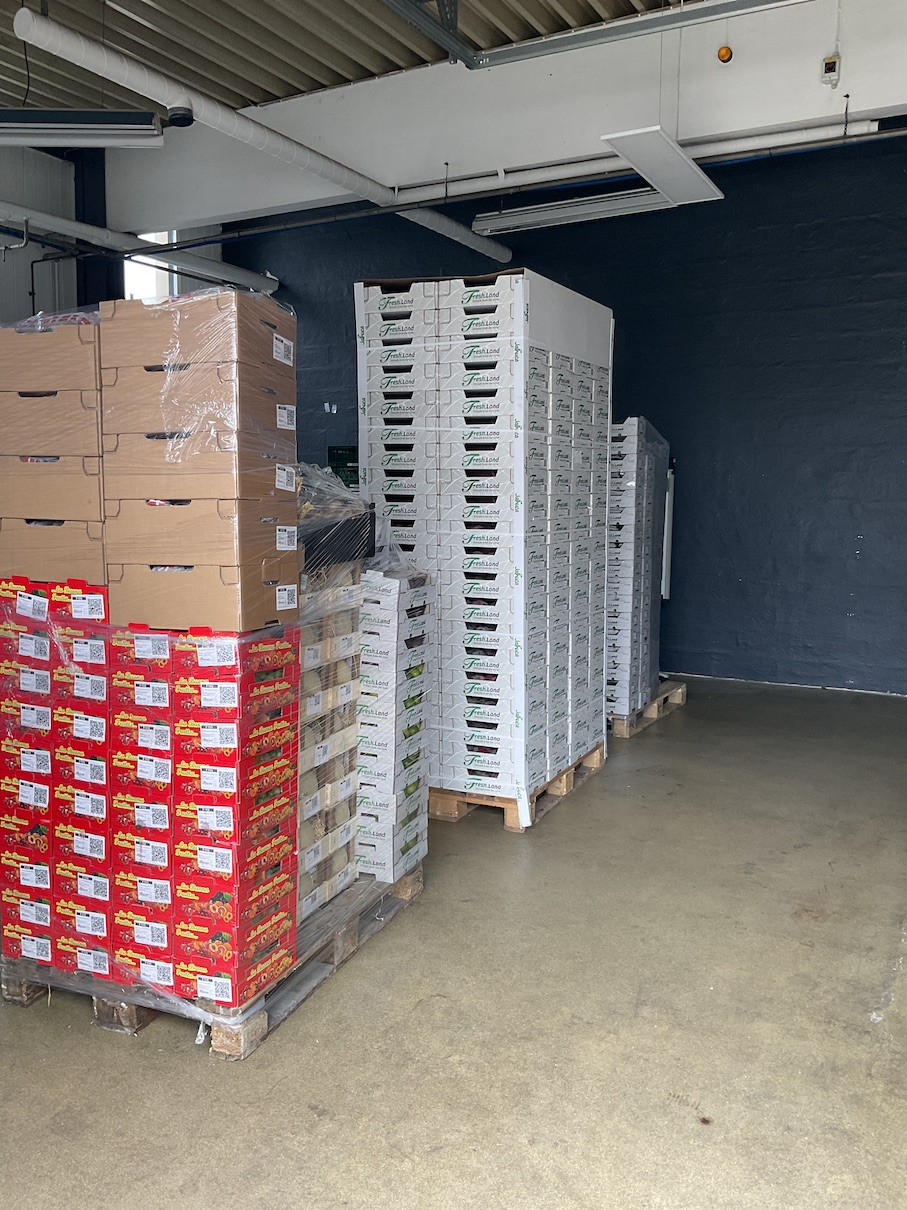
\includegraphics[width=0.32\textwidth,height=\textheight]{./figures/chainge_image1.jpeg}}\hfill
\subfloat[]{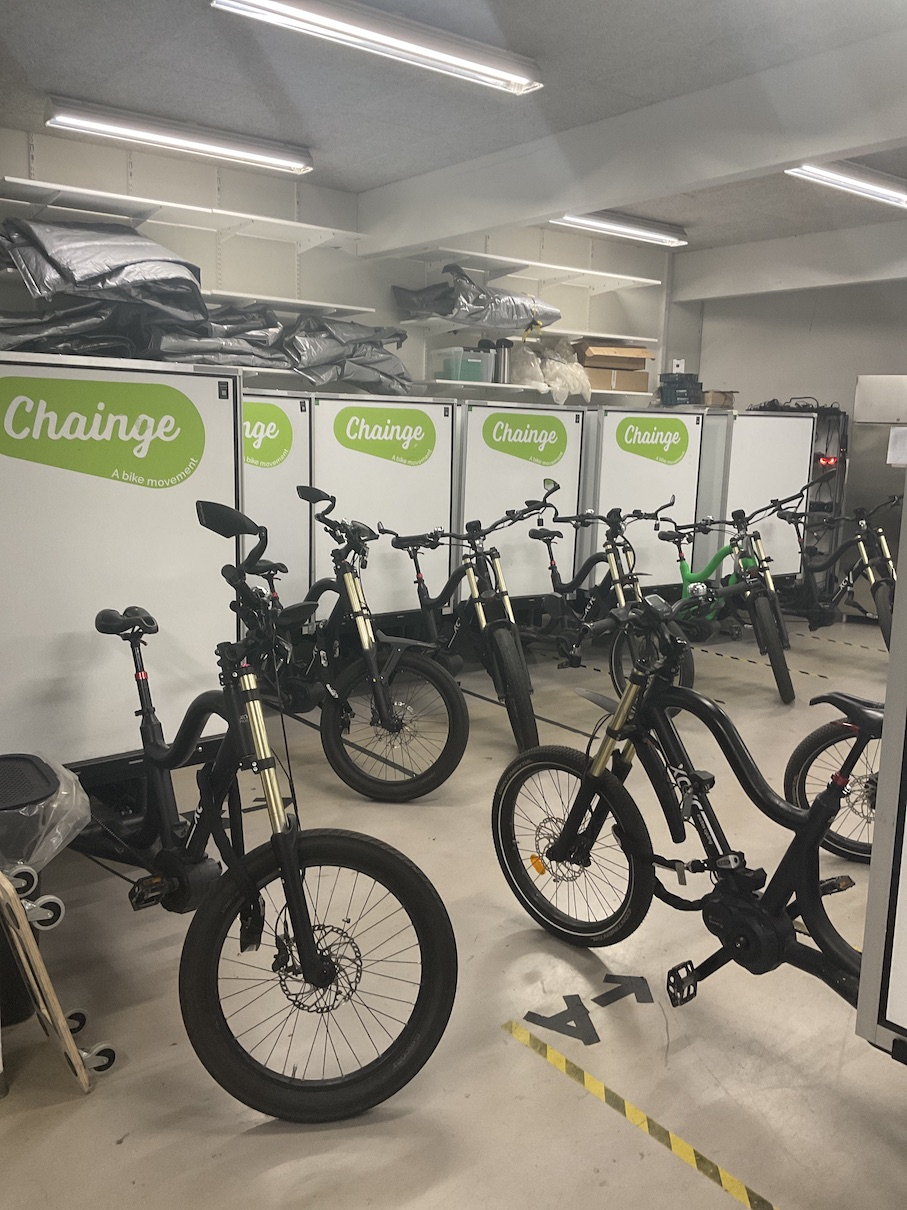
\includegraphics[width=0.32\textwidth,height=\textheight]{./figures/chainge_image2.jpeg}}\hfill
\subfloat[]{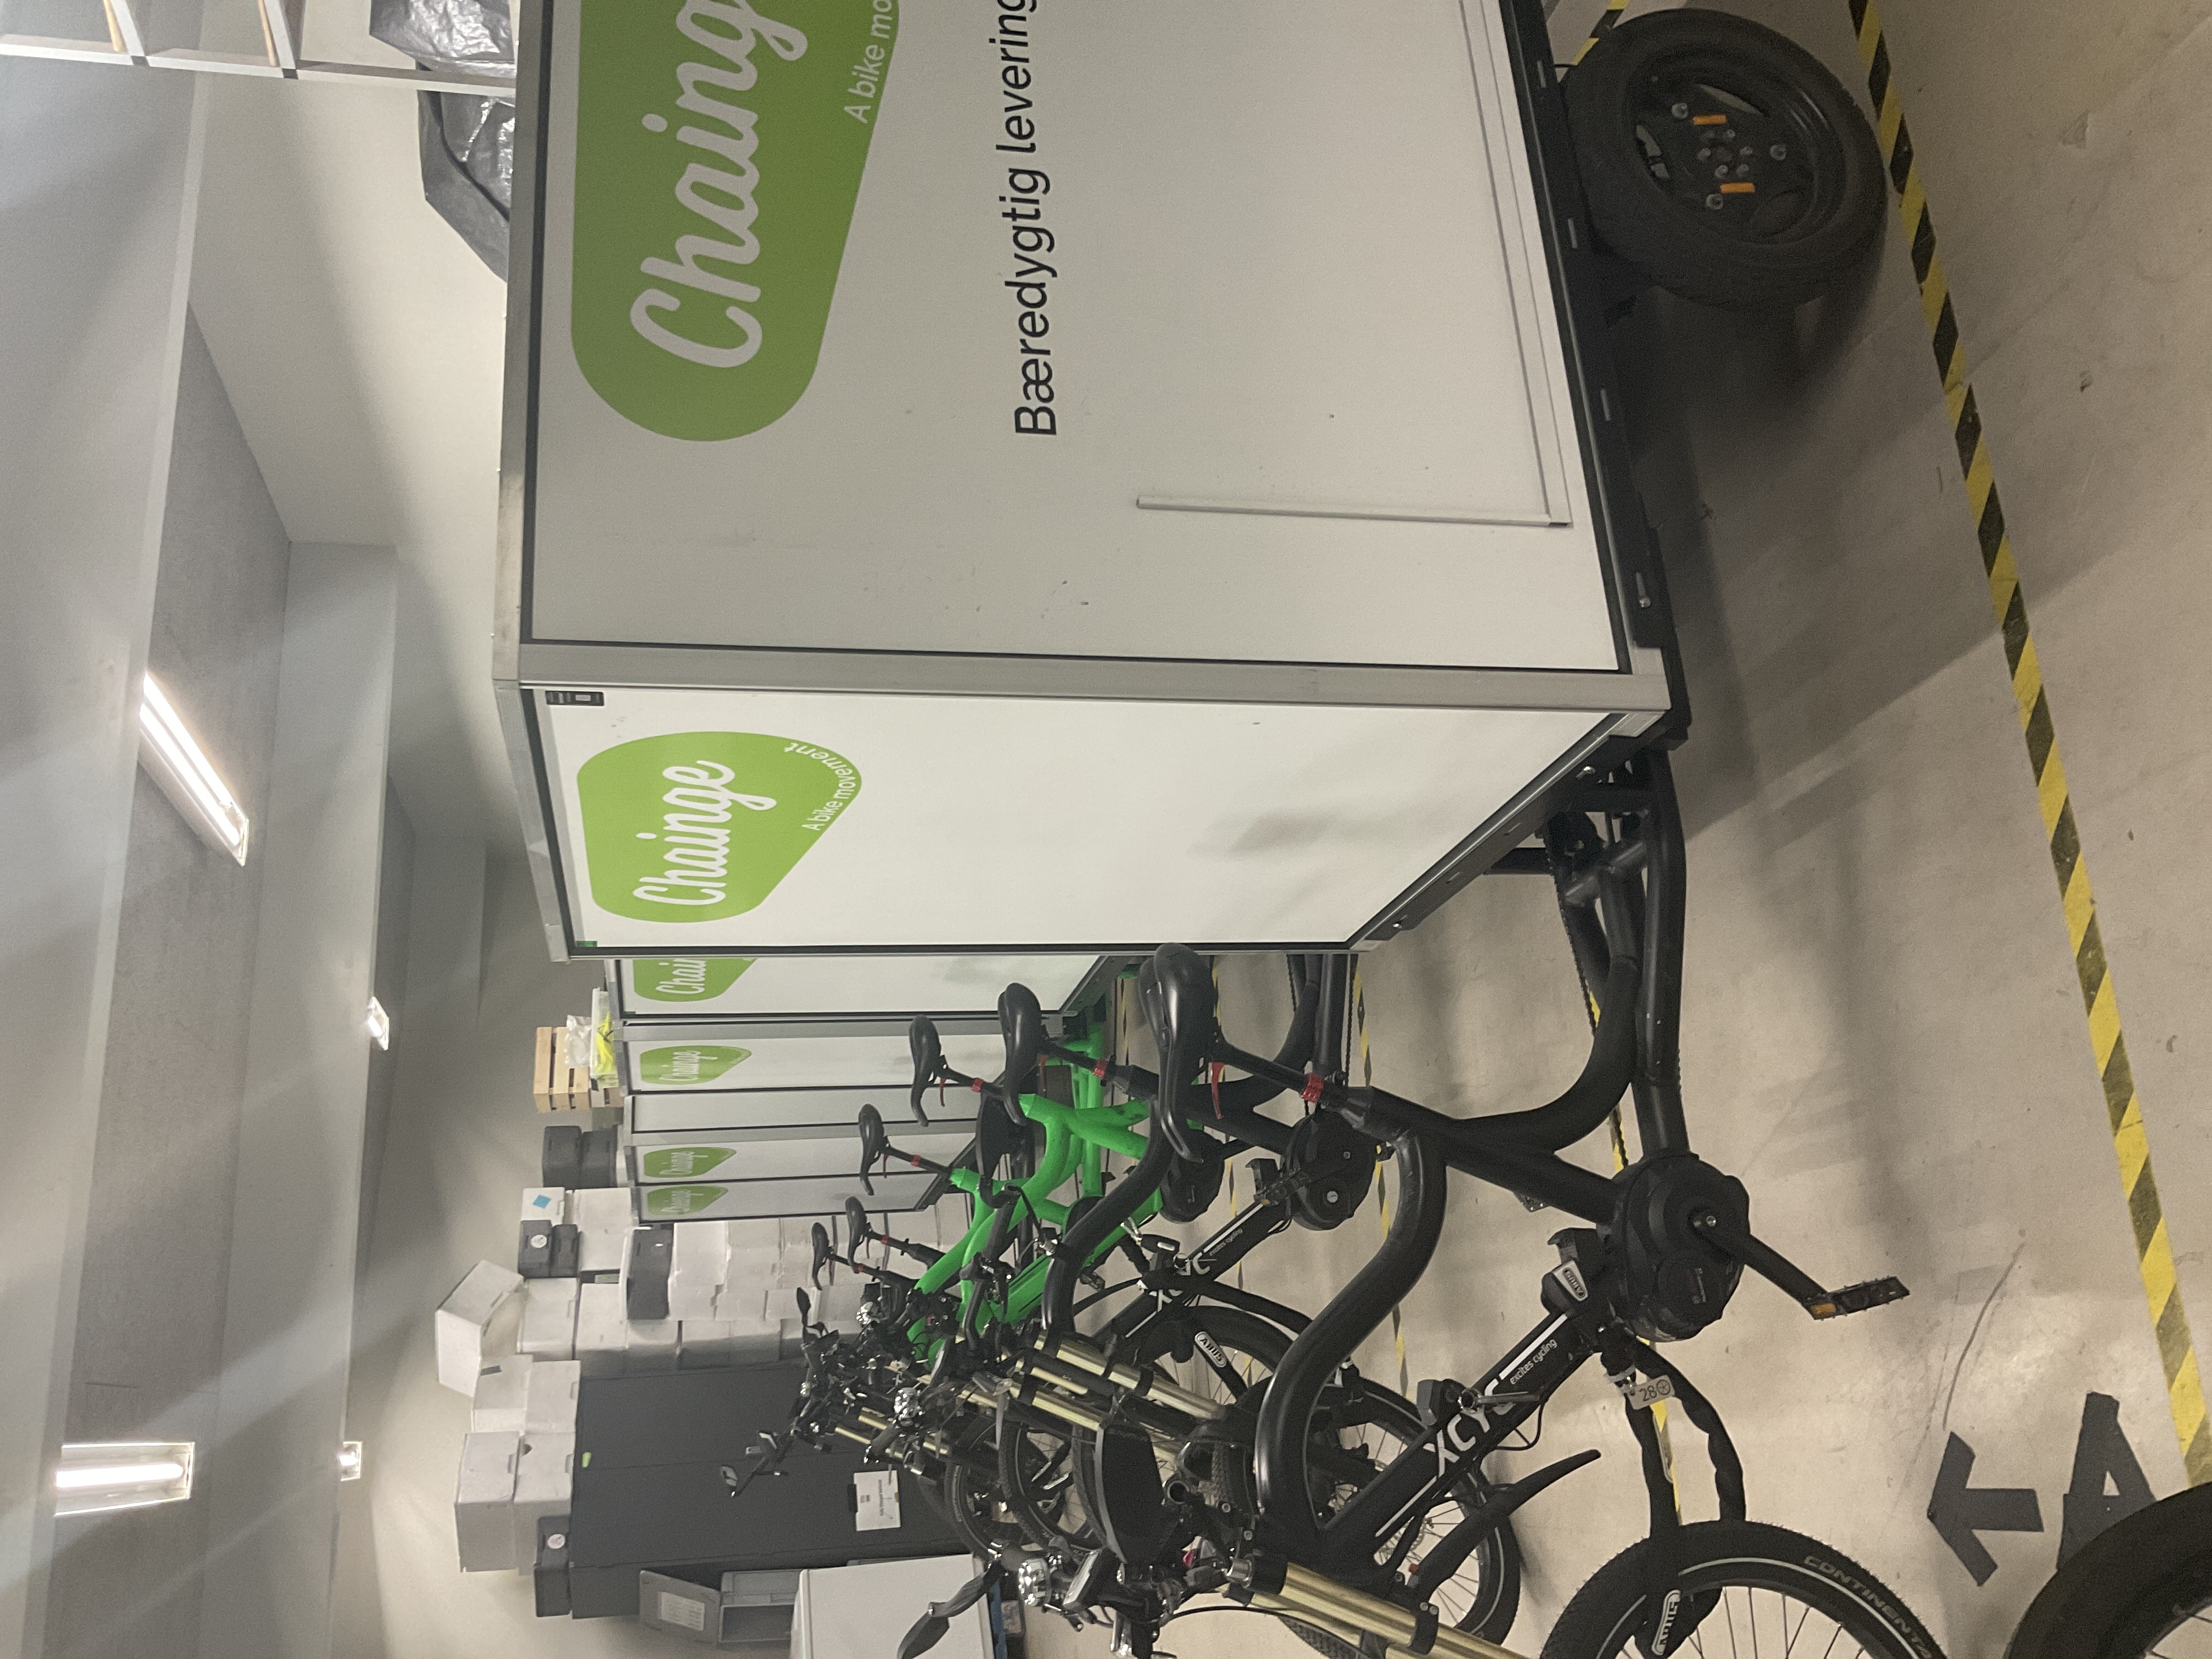
\includegraphics[width=0.32\textwidth,height=\textheight]{./figures/chainge_image3.jpeg}}

\subfloat[]{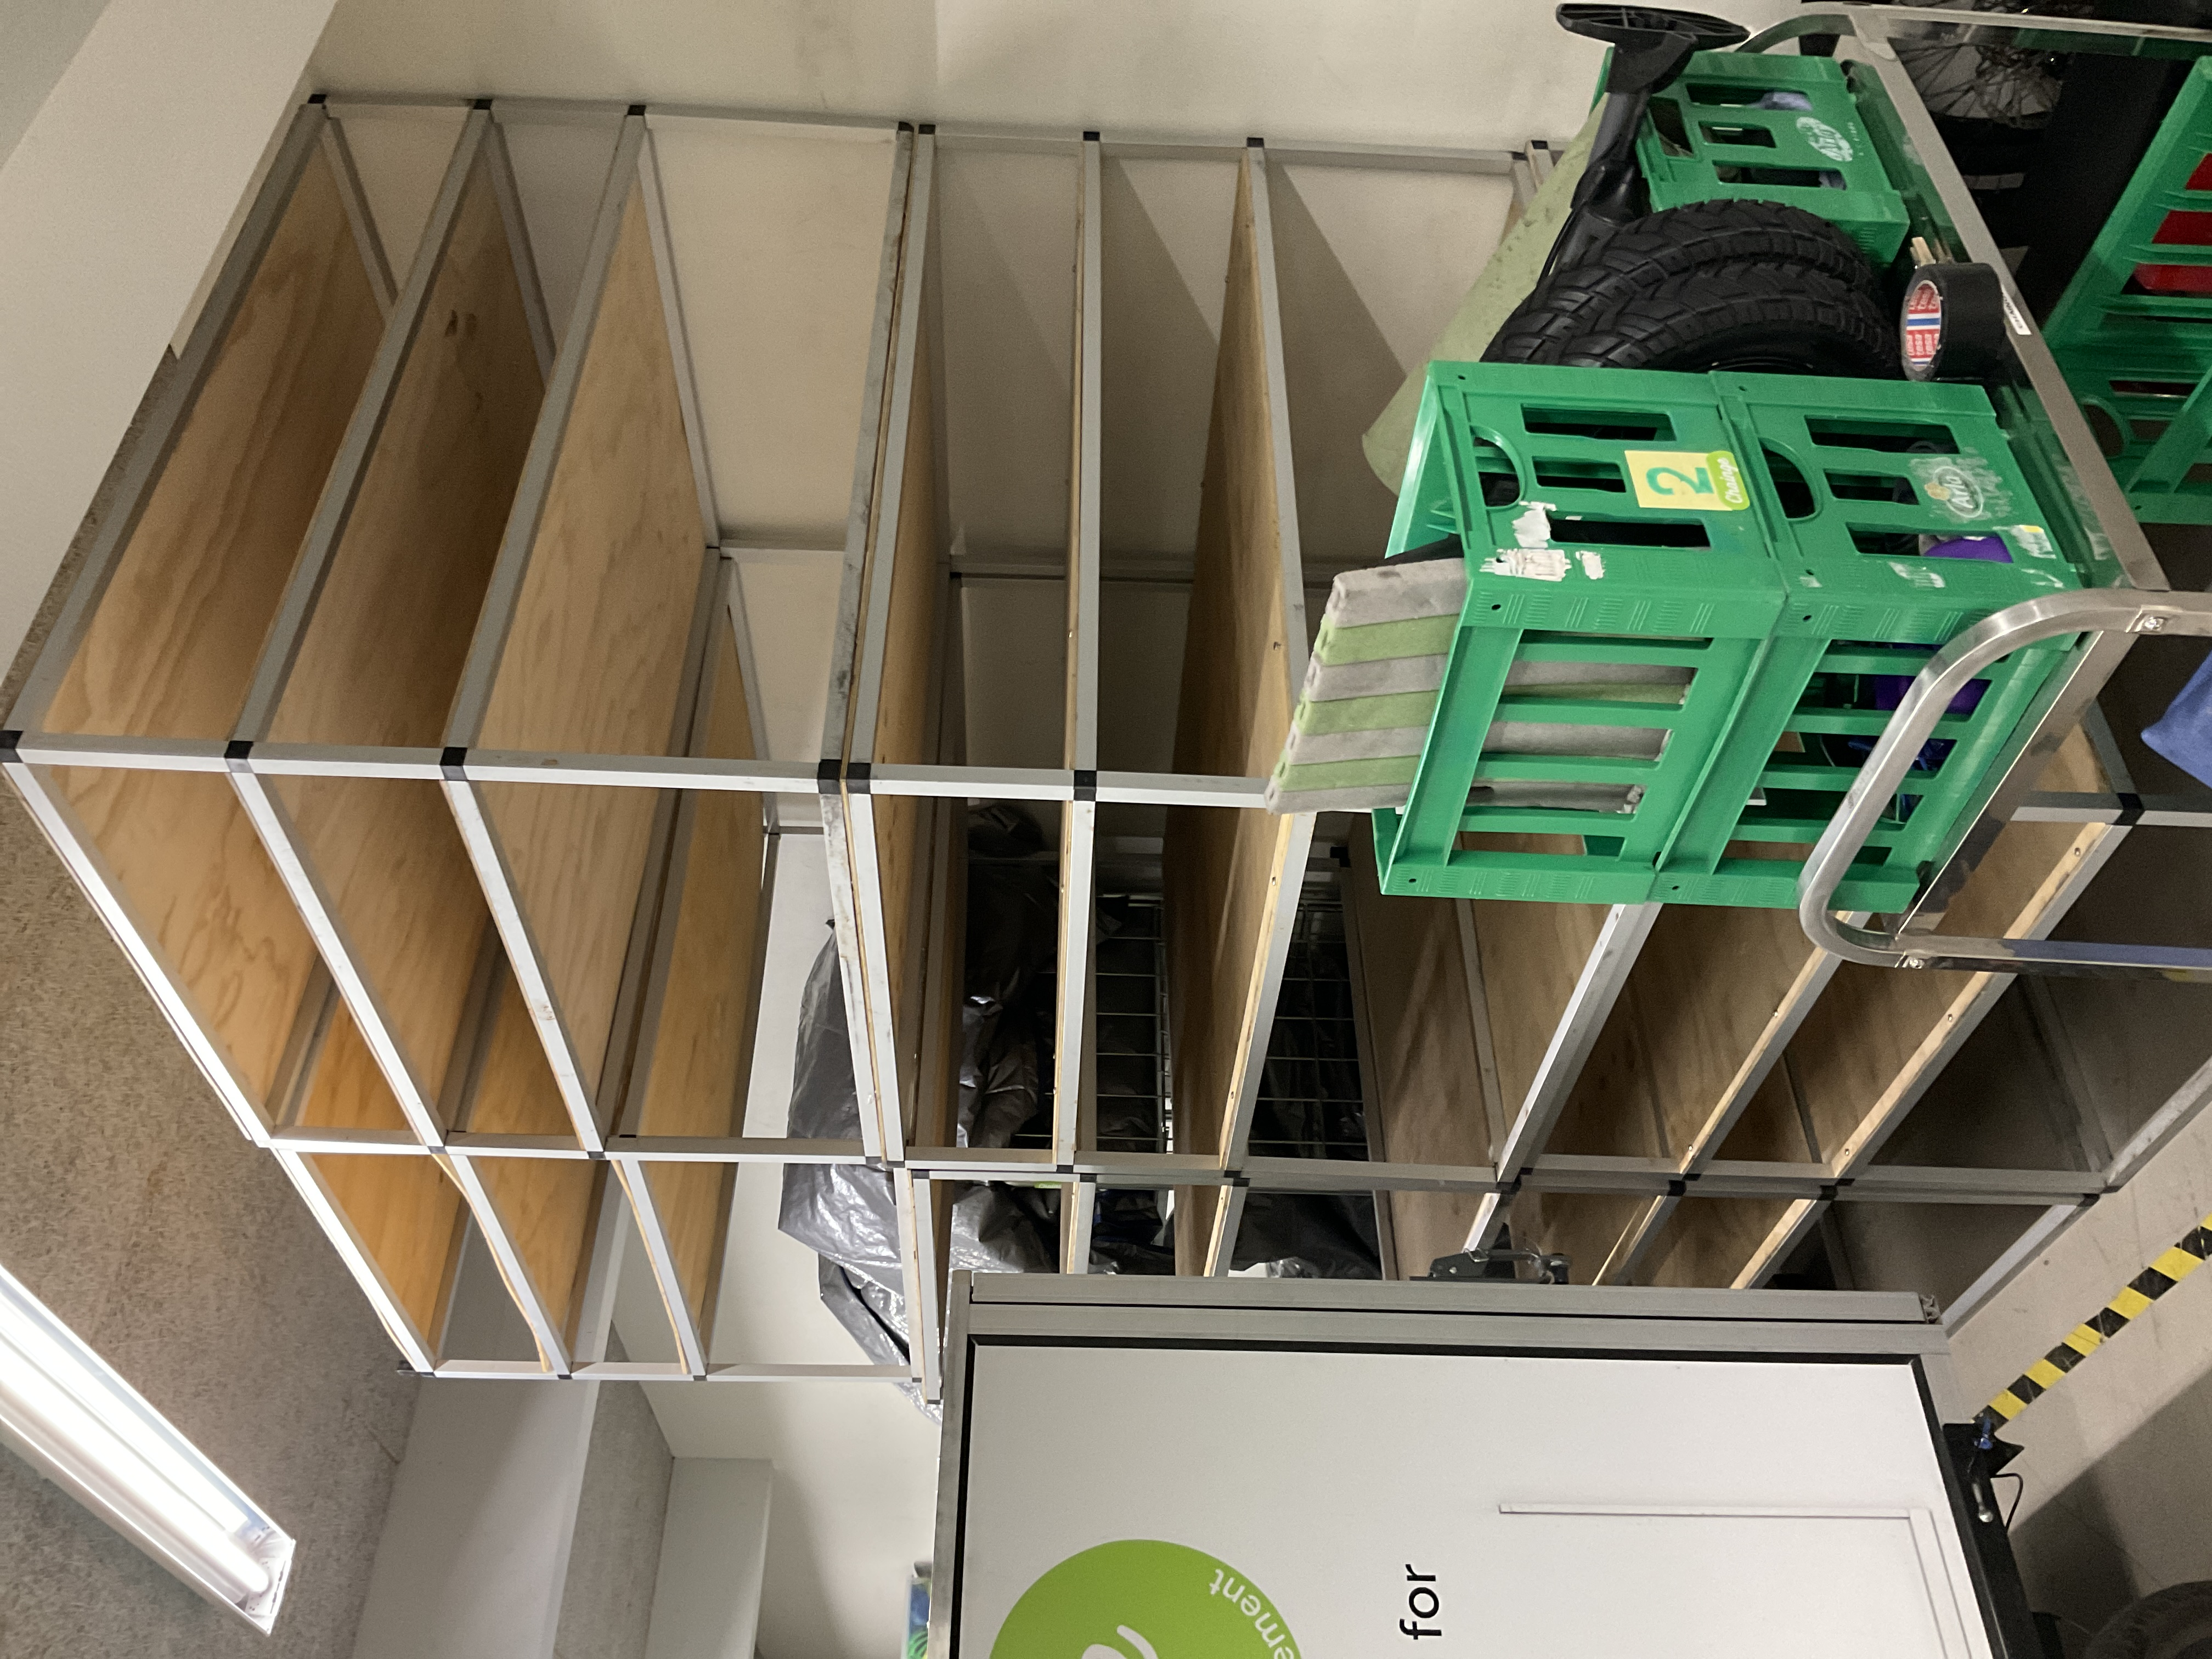
\includegraphics[width=0.32\textwidth,height=\textheight]{./figures/chainge_image4.jpeg}}\hfill
\subfloat[]{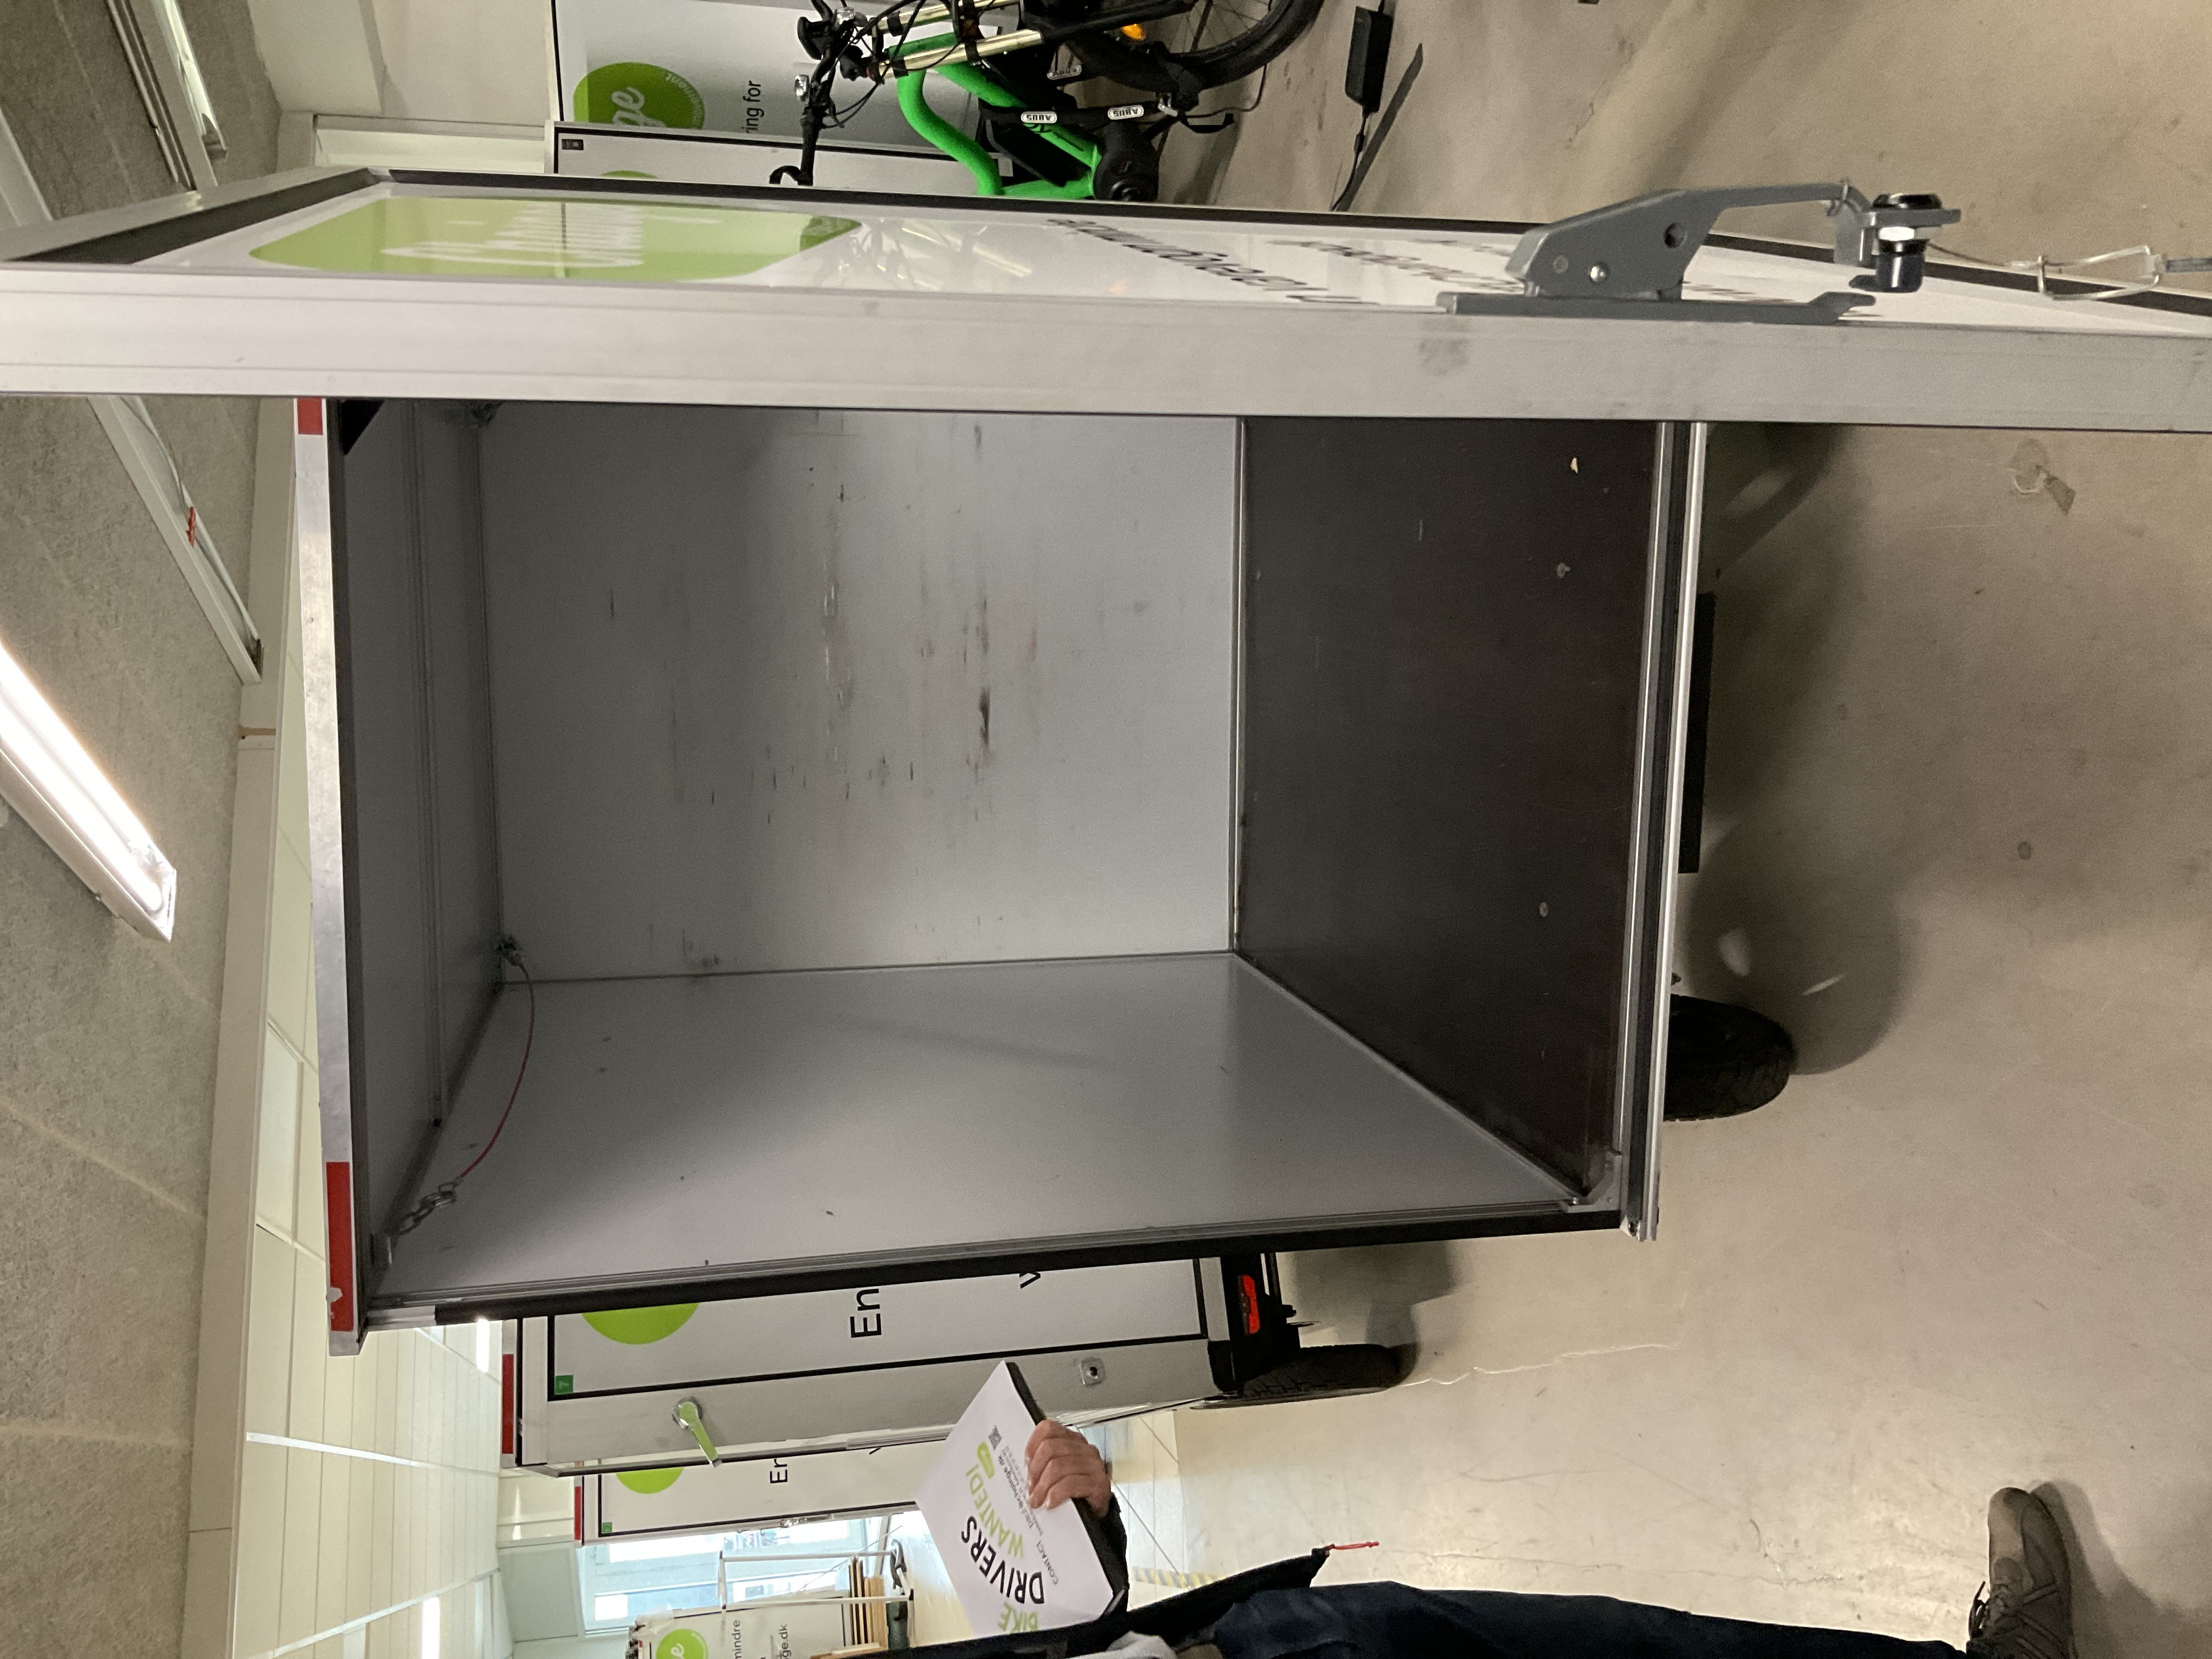
\includegraphics[width=0.32\textwidth,height=\textheight]{./figures/chainge_image5.jpeg}}\hfill
\subfloat[]{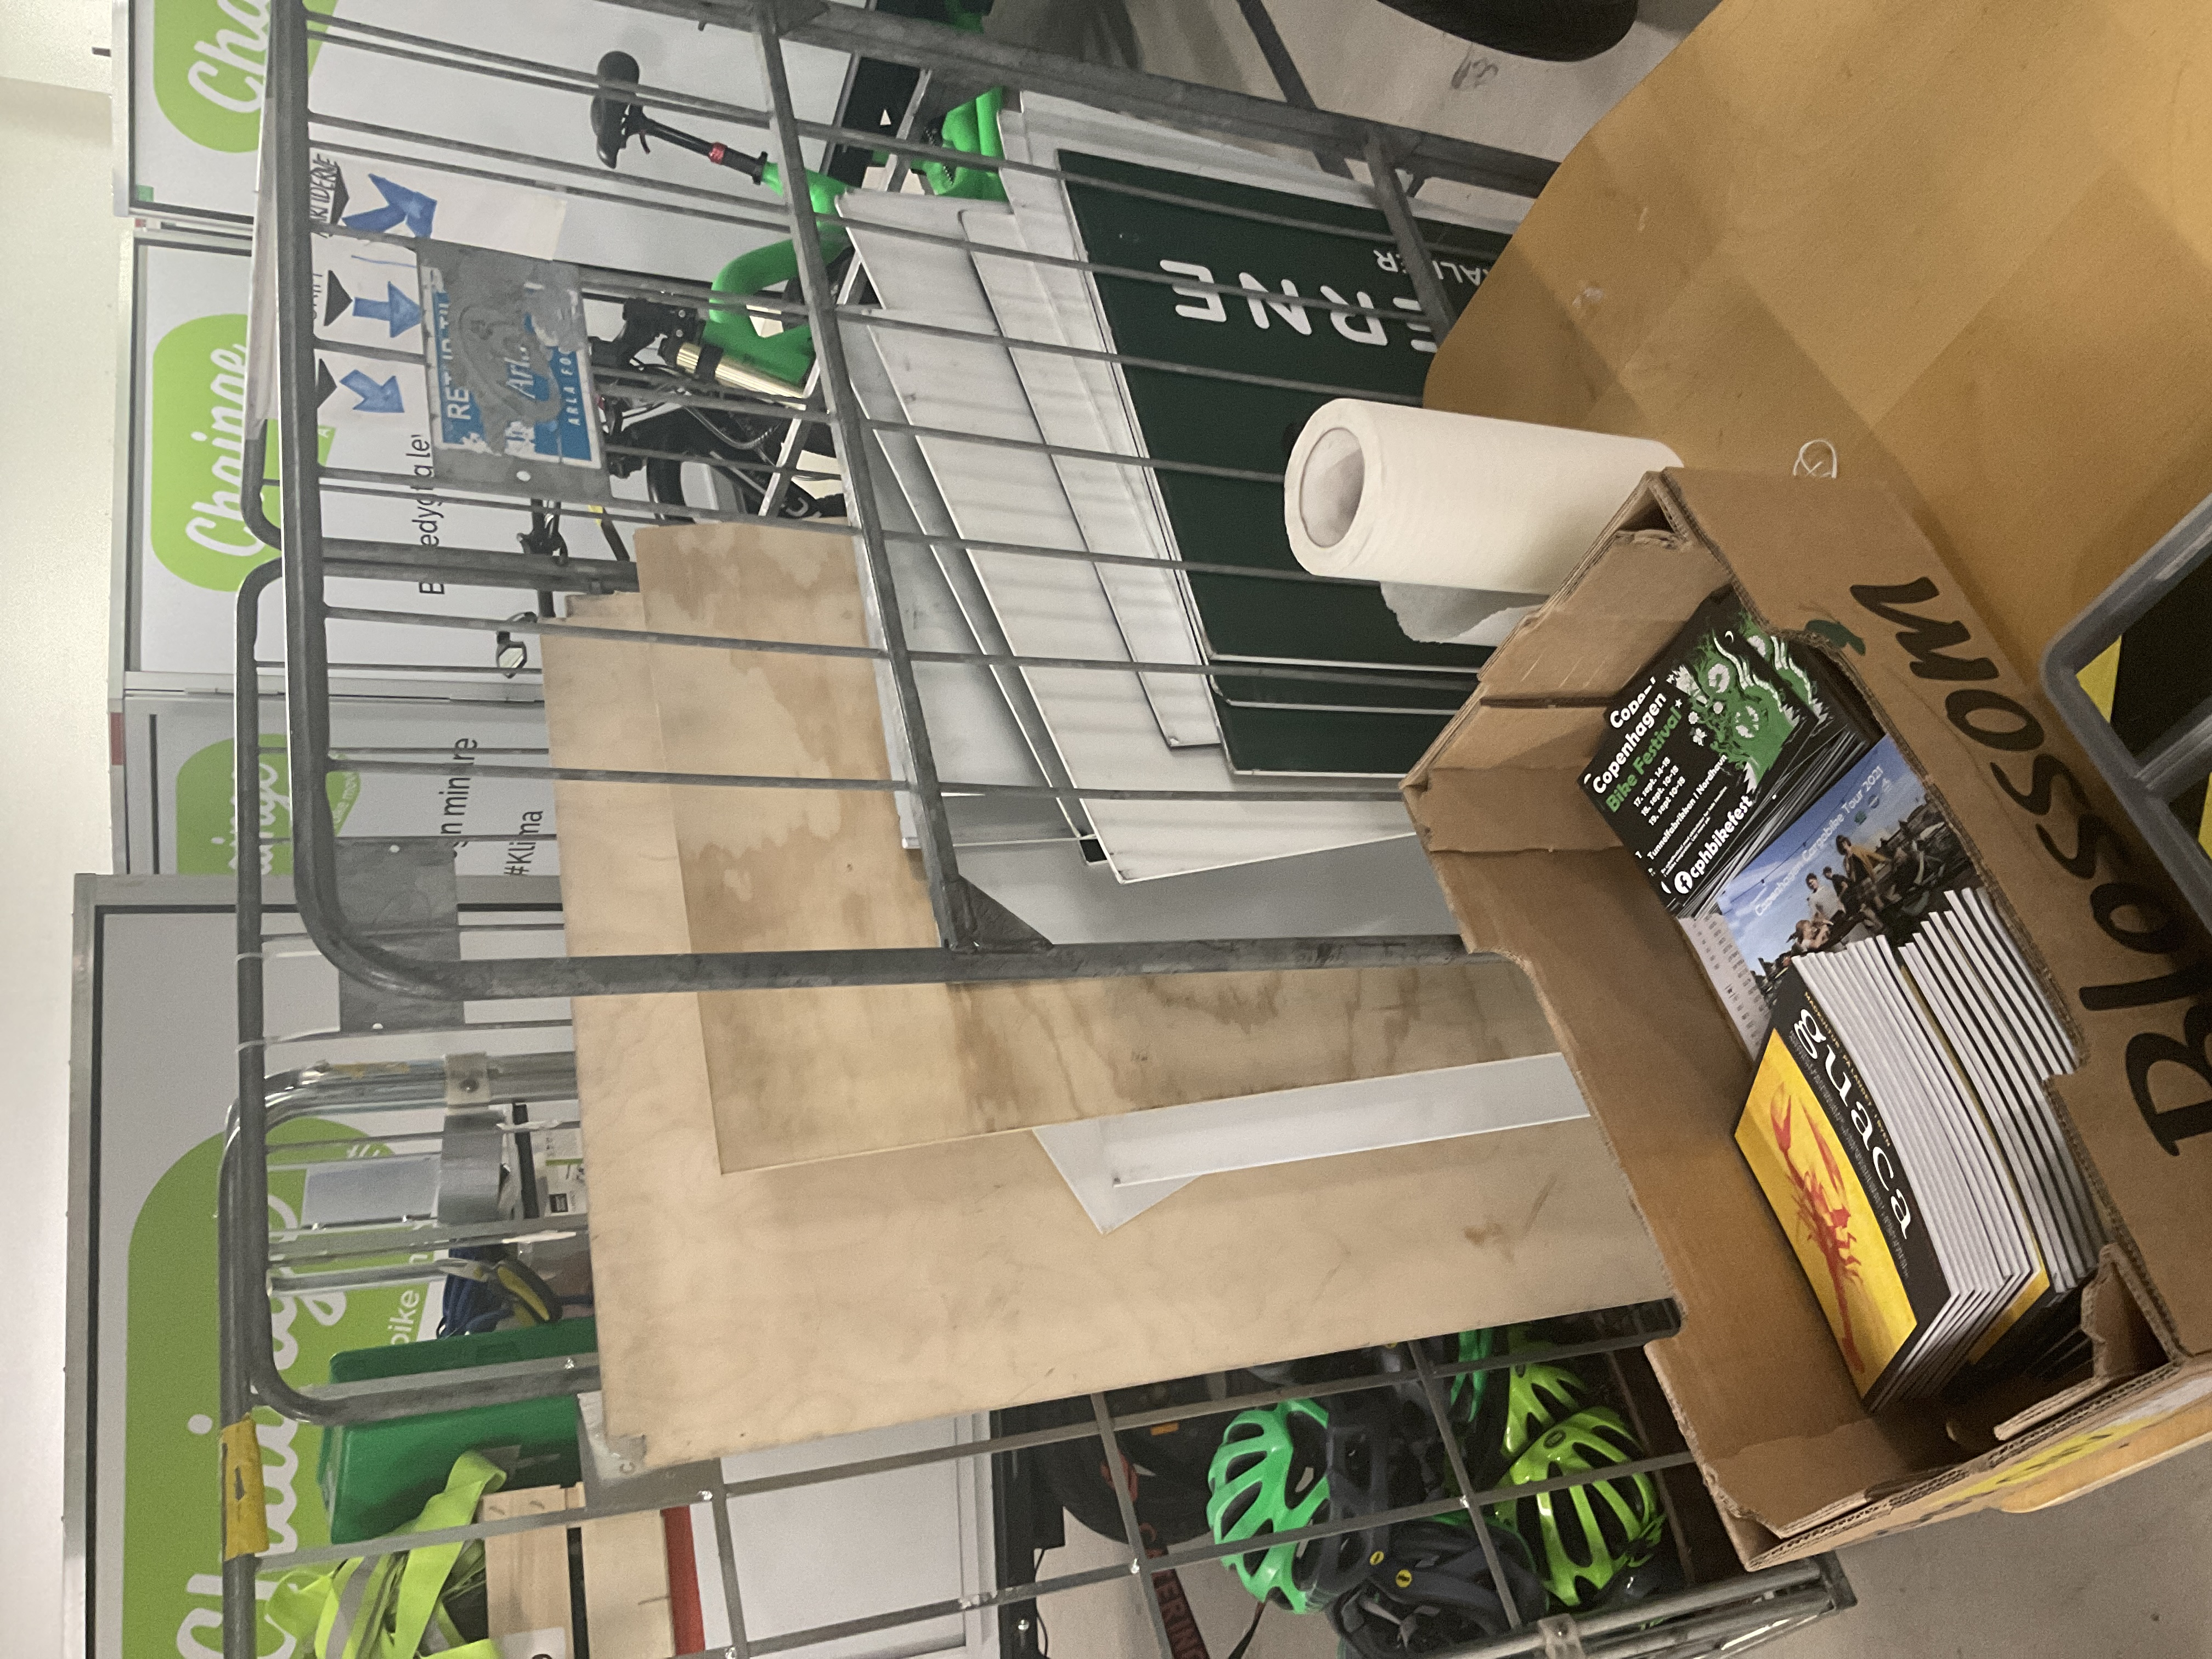
\includegraphics[width=0.32\textwidth,height=\textheight]{./figures/chainge_image6.jpeg}}

\caption[{Subfigures caption}]{Subfigures caption}

\label{fig:chainge_headquarters}

\end{pandoccrossrefsubfigures}

We wanted to interview Drivers working at Chainge to learn more about
their work tasks and the onboarding process. Torben from Chainge
assisted in arranging interviews with newly hired Drivers a week later.
We wanted to interview Drivers that had recently experienced the
onboarding process or were in the middle of the onboarding. We conducted
three interviews with new Drivers that had worked at Chainge for less
than four weeks. The three Drivers had worked at Chainge for one week,
two weeks and three weeks respectively.

The interviews were conducted at Chainge's headquarters to make it
convenient for the interviewees. Prior to the interviews, we created an
interview guide to structure and facilitate the interviews. This guide
was semi-structured, which is more flexible for structured interviews
but not as loosely structured as unstructured interviews (Bryman, 2012).
The interview guide provided flexibility for questions that suddenly
arose but at the same time managed the interview in a way so we did not
deviate from the planned questions. We gained a lot of knowledge from
the interviews. One incident during one of the interviews was
particularly interesting. When the interviewee was asked about
challenges related to job tasks, she referred to a situation where the
recipient was not home to receive the package. Instead of bringing the
package to the headquarters, she went back later on her delivery route
to try and deliver the package again (Interview 3). The interviewer that
conducted the interview would probably not have paid special interest in
the statement if Torben had not explained the standard procedure some
days in advance. The standard way of working is to only try to deliver
the packages once and if nobody is at the designated location, then the
package is to be brought to the headquarter. This example together with
the other interviews shed light on the need for an improved and
structured onboarding process focussing on communication.

\hypertarget{sec:colour_coding}{%
\subsection{Colour coding of data}\label{sec:colour_coding}}

Numerous frameworks and tools exist for grouping interview data in
categories. We chose an accessible and visual methodological approach of
highlighting words and sentences with colors, each color corresponding
to a category in our coding format table (Appendix 2). Figure 1
illustrates the colours and the corresponding definitions:

\begin{longtable}[]{@{}ll@{}}
\toprule
Colour & Definition \\
\midrule
\endhead
Green & Positive aspects of the Drivers' job \\
Yellow & General knowledge about work practices \\
Red & Challenges/insecurities experienced by Drivers \\
\bottomrule
\end{longtable}

\emph{Figure 1: Colour Coding Table}

This approach is inspired by Grounded Theory, which advocates for
grounding research approaches in empirical data at every step of the
process (Charmaz, 1996). Grounded Theory advocates not only leveraging
interview data as a source of knowledge, but also as a starting point
for conducting further ethnographic research. This is known as deductive
determination, wherein the research focus is determined by deducing the
main points in the data (Charmaz, 1996).

The aim is to improve the onboarding by structuring relevant information
for the Drivers. We decided to highlight data in relation to the
different categories to prioritise information relevant for the final
solution. The three color codings were chosen, as we would be able to
clearly highly positive aspects of the onboarding process that should
not changed (green code), information that might be needed in the
corresponding solution (yellow code) and challenges and/or insecurities
that need to be addressed in the onboarding process (red code).

\hypertarget{sec:participant_obs}{%
\subsection{Participant observation}\label{sec:participant_obs}}

As part of our empirical gathering, we have conducted participant
observation. Spradley (1980) has categorised different degrees of
participant observation. We utilised the type of participation
classified as passive participation. Spradley (1980) applies the
insider/outsider perspective to explain the degree of participation.

The person being observed was one of the interview respondents that was
also a newly hired Driver. This observation was arranged during our
interview with the Driver. The Driver agreed to being observed while
driving a delivery route for Chainge. The Driver was followed on bike by
two of the students from the group and was observed while performing his
work tasks. The students did not seek to maintain a balance between an
insider/outsider perspective as they merely behaved as outsiders to
observe from the outside. The students drove after the Driver so they
were present at the scene but they did not participate in performing the
work tasks. We decided to pursue participant observation with the aim of
exploring tacit knowledge about the work tasks that was not vocalised
during the interview.

Additionally, we wanted to take pictures and videos as they could be
useful later on and as a point of reference for the remaining students
that did not participate.

\textbf{START images of driver shadowing}

\begin{pandoccrossrefsubfigures}

\subfloat[]{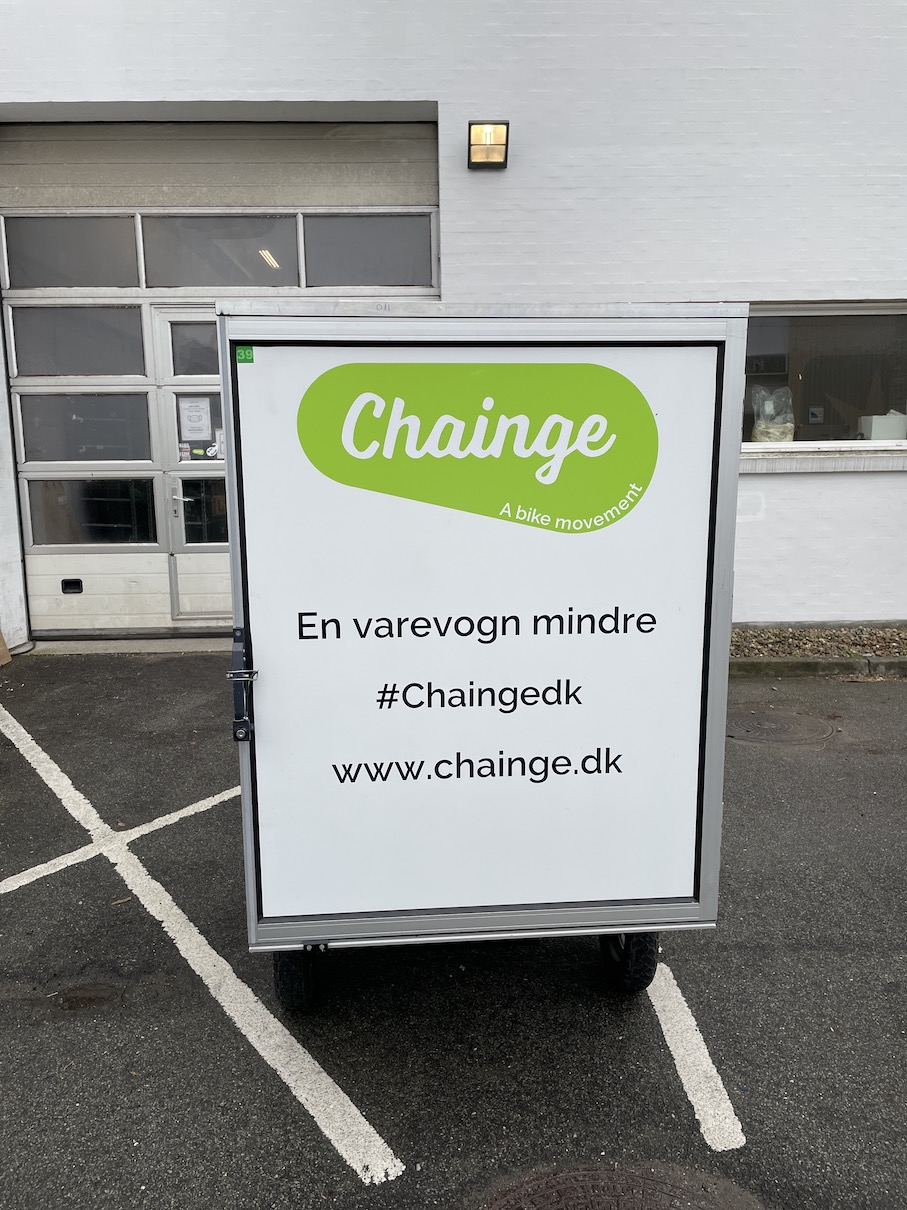
\includegraphics[width=0.49\textwidth,height=\textheight]{./figures/driver_image1.jpeg}}\hfill
\subfloat[]{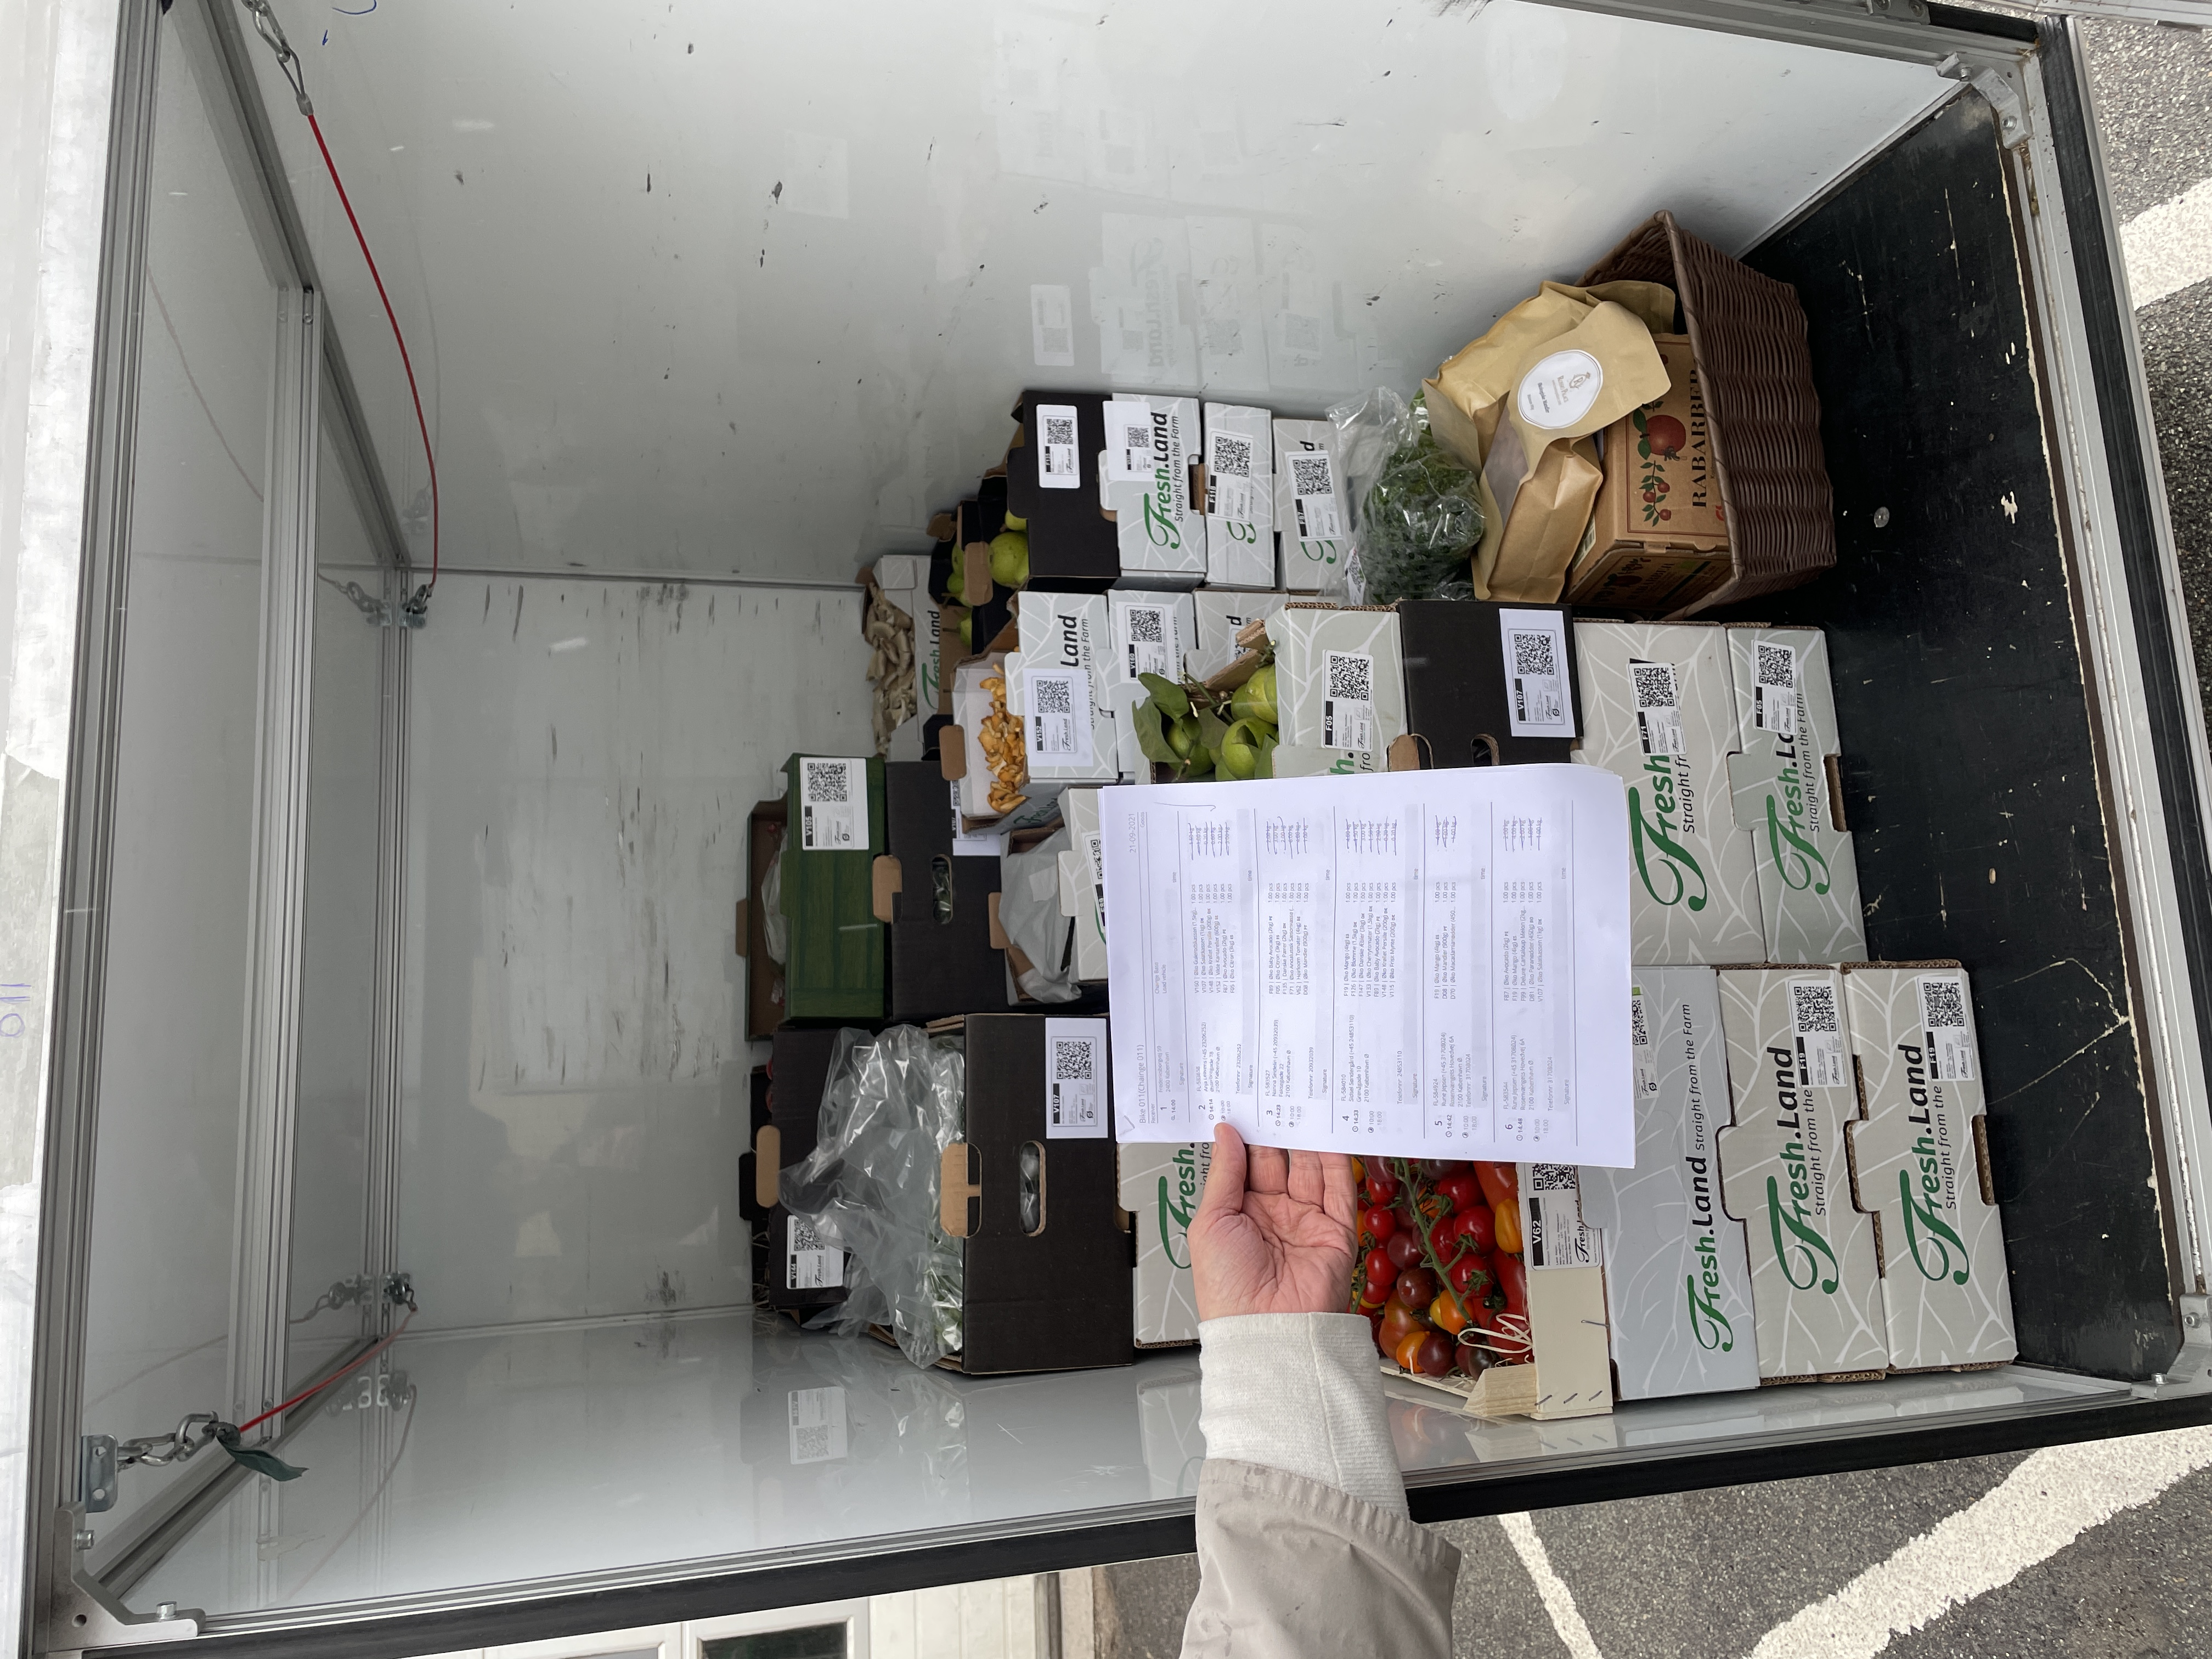
\includegraphics[width=0.49\textwidth,height=\textheight]{./figures/driver_image2.jpeg}}

\caption[{Subfigures caption}]{Subfigures caption}

\label{fig:chainge_driver}

\end{pandoccrossrefsubfigures}

\textbf{END images of driver shadowing}

We experienced an interesting situation before we jumped on our bikes to
tag along the Driver. At the headquarter, we observed a manager
conveying a large amount of information to a small group of new Drivers
on how to deliver packages to a customer.

\hypertarget{sec:ideation_workshop}{%
\subsection{Ideation workshop}\label{sec:ideation_workshop}}

Grounded in the themes identified through our category-coded interview
data, we conducted an internal ideation workshop with brainstorming as
the main focus, wherein we explored the hedonic qualities of design
openings and potential solutions. Our approach was to ignore the
technological possibilities in situ, as well as any constraints,
leveraging a user-centric approach instead. In this process we
emphasised the hedonic benefits a solution would have on Chainge
employees, with basis in the problems they vocalised in our interviews .

Kolko (2018) describes how brainstorming emerged as a playful and
creative way of problem solving. Four principles are relevant in a
brainstorming session: to avoid criticisms, encourage crazy ideas,
produce a variety of ideas and utilise the ideas from the team members
to build upon to extend ideas (Kolko, 2018). According to Kolko (2018),
empathy is the foundation in participatory design practice.

We brainstormed themes on a whiteboard to figure out what should
characterise the solution. Afterwards, we individually marked three
words each that we found the most important. It became evident through
this process that the central theme of our solution should be the
existence and contextual accessibility of structured, standardised
information on work practices and responsibilities for Chainge drivers.
We have strived to be empathic in the brainstorming within the group to
be open-minded and explorative when being presented to ideas.

\textbf{START images of brainstorming}

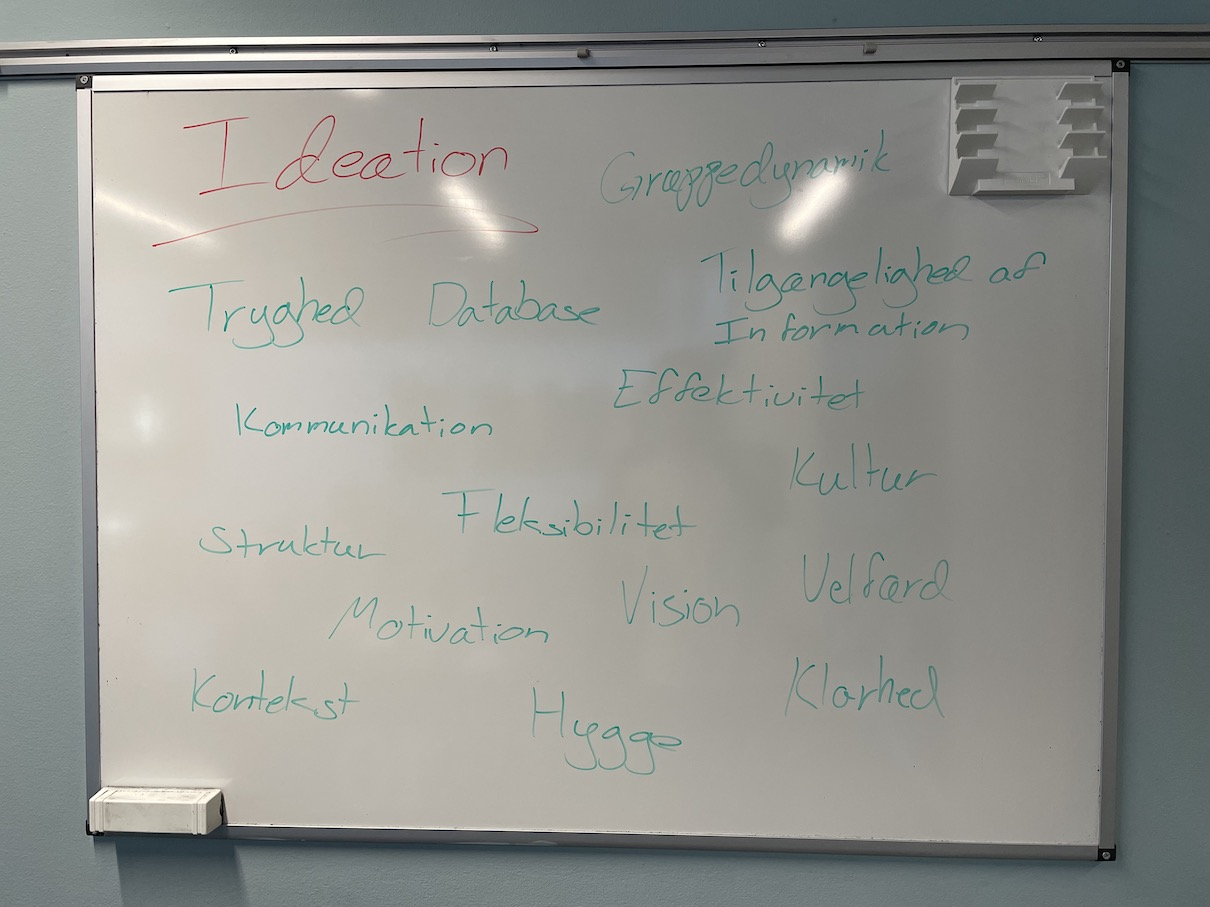
\includegraphics[width=0.32\textwidth,height=\textheight]{./figures/brainstorm_image1.jpg}
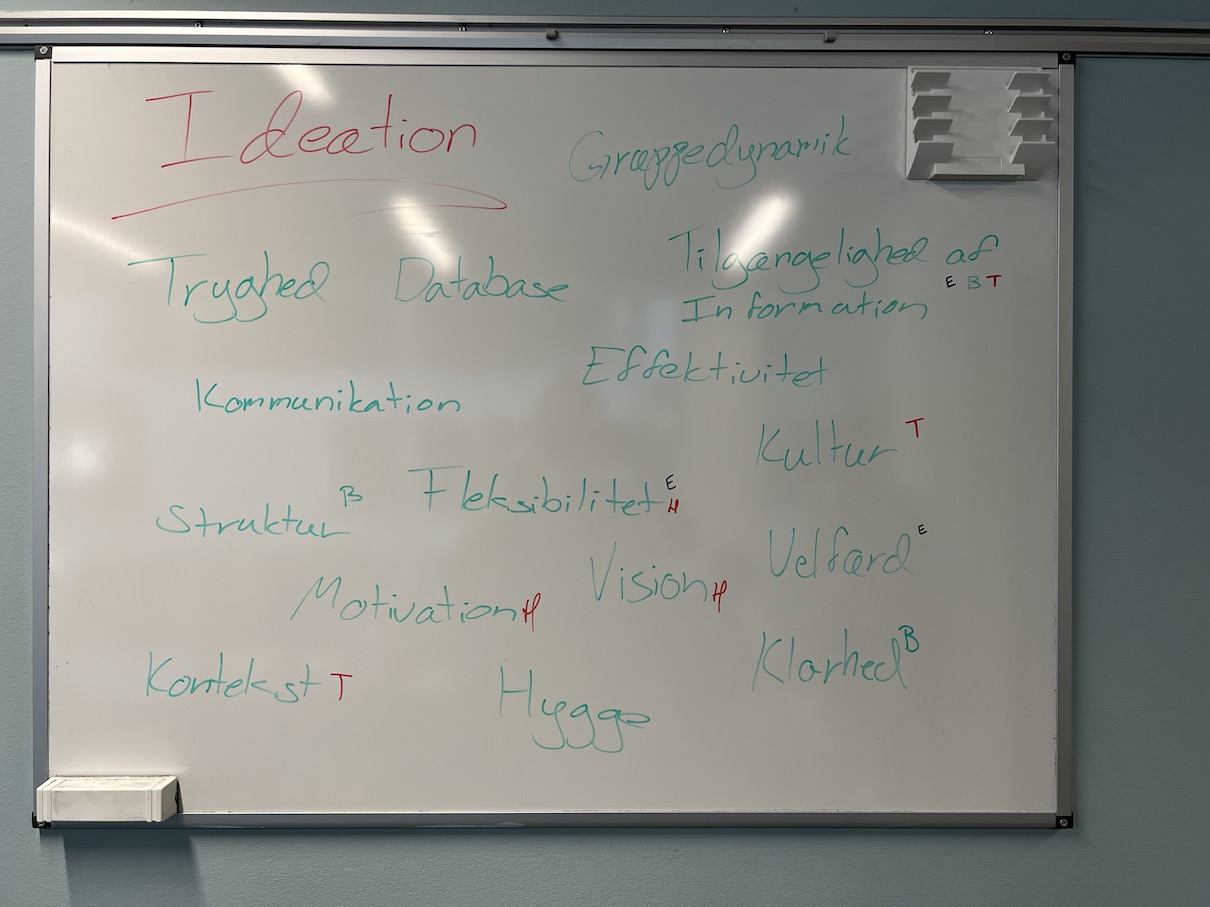
\includegraphics[width=0.32\textwidth,height=\textheight]{./figures/brainstorm_image2.jpg}
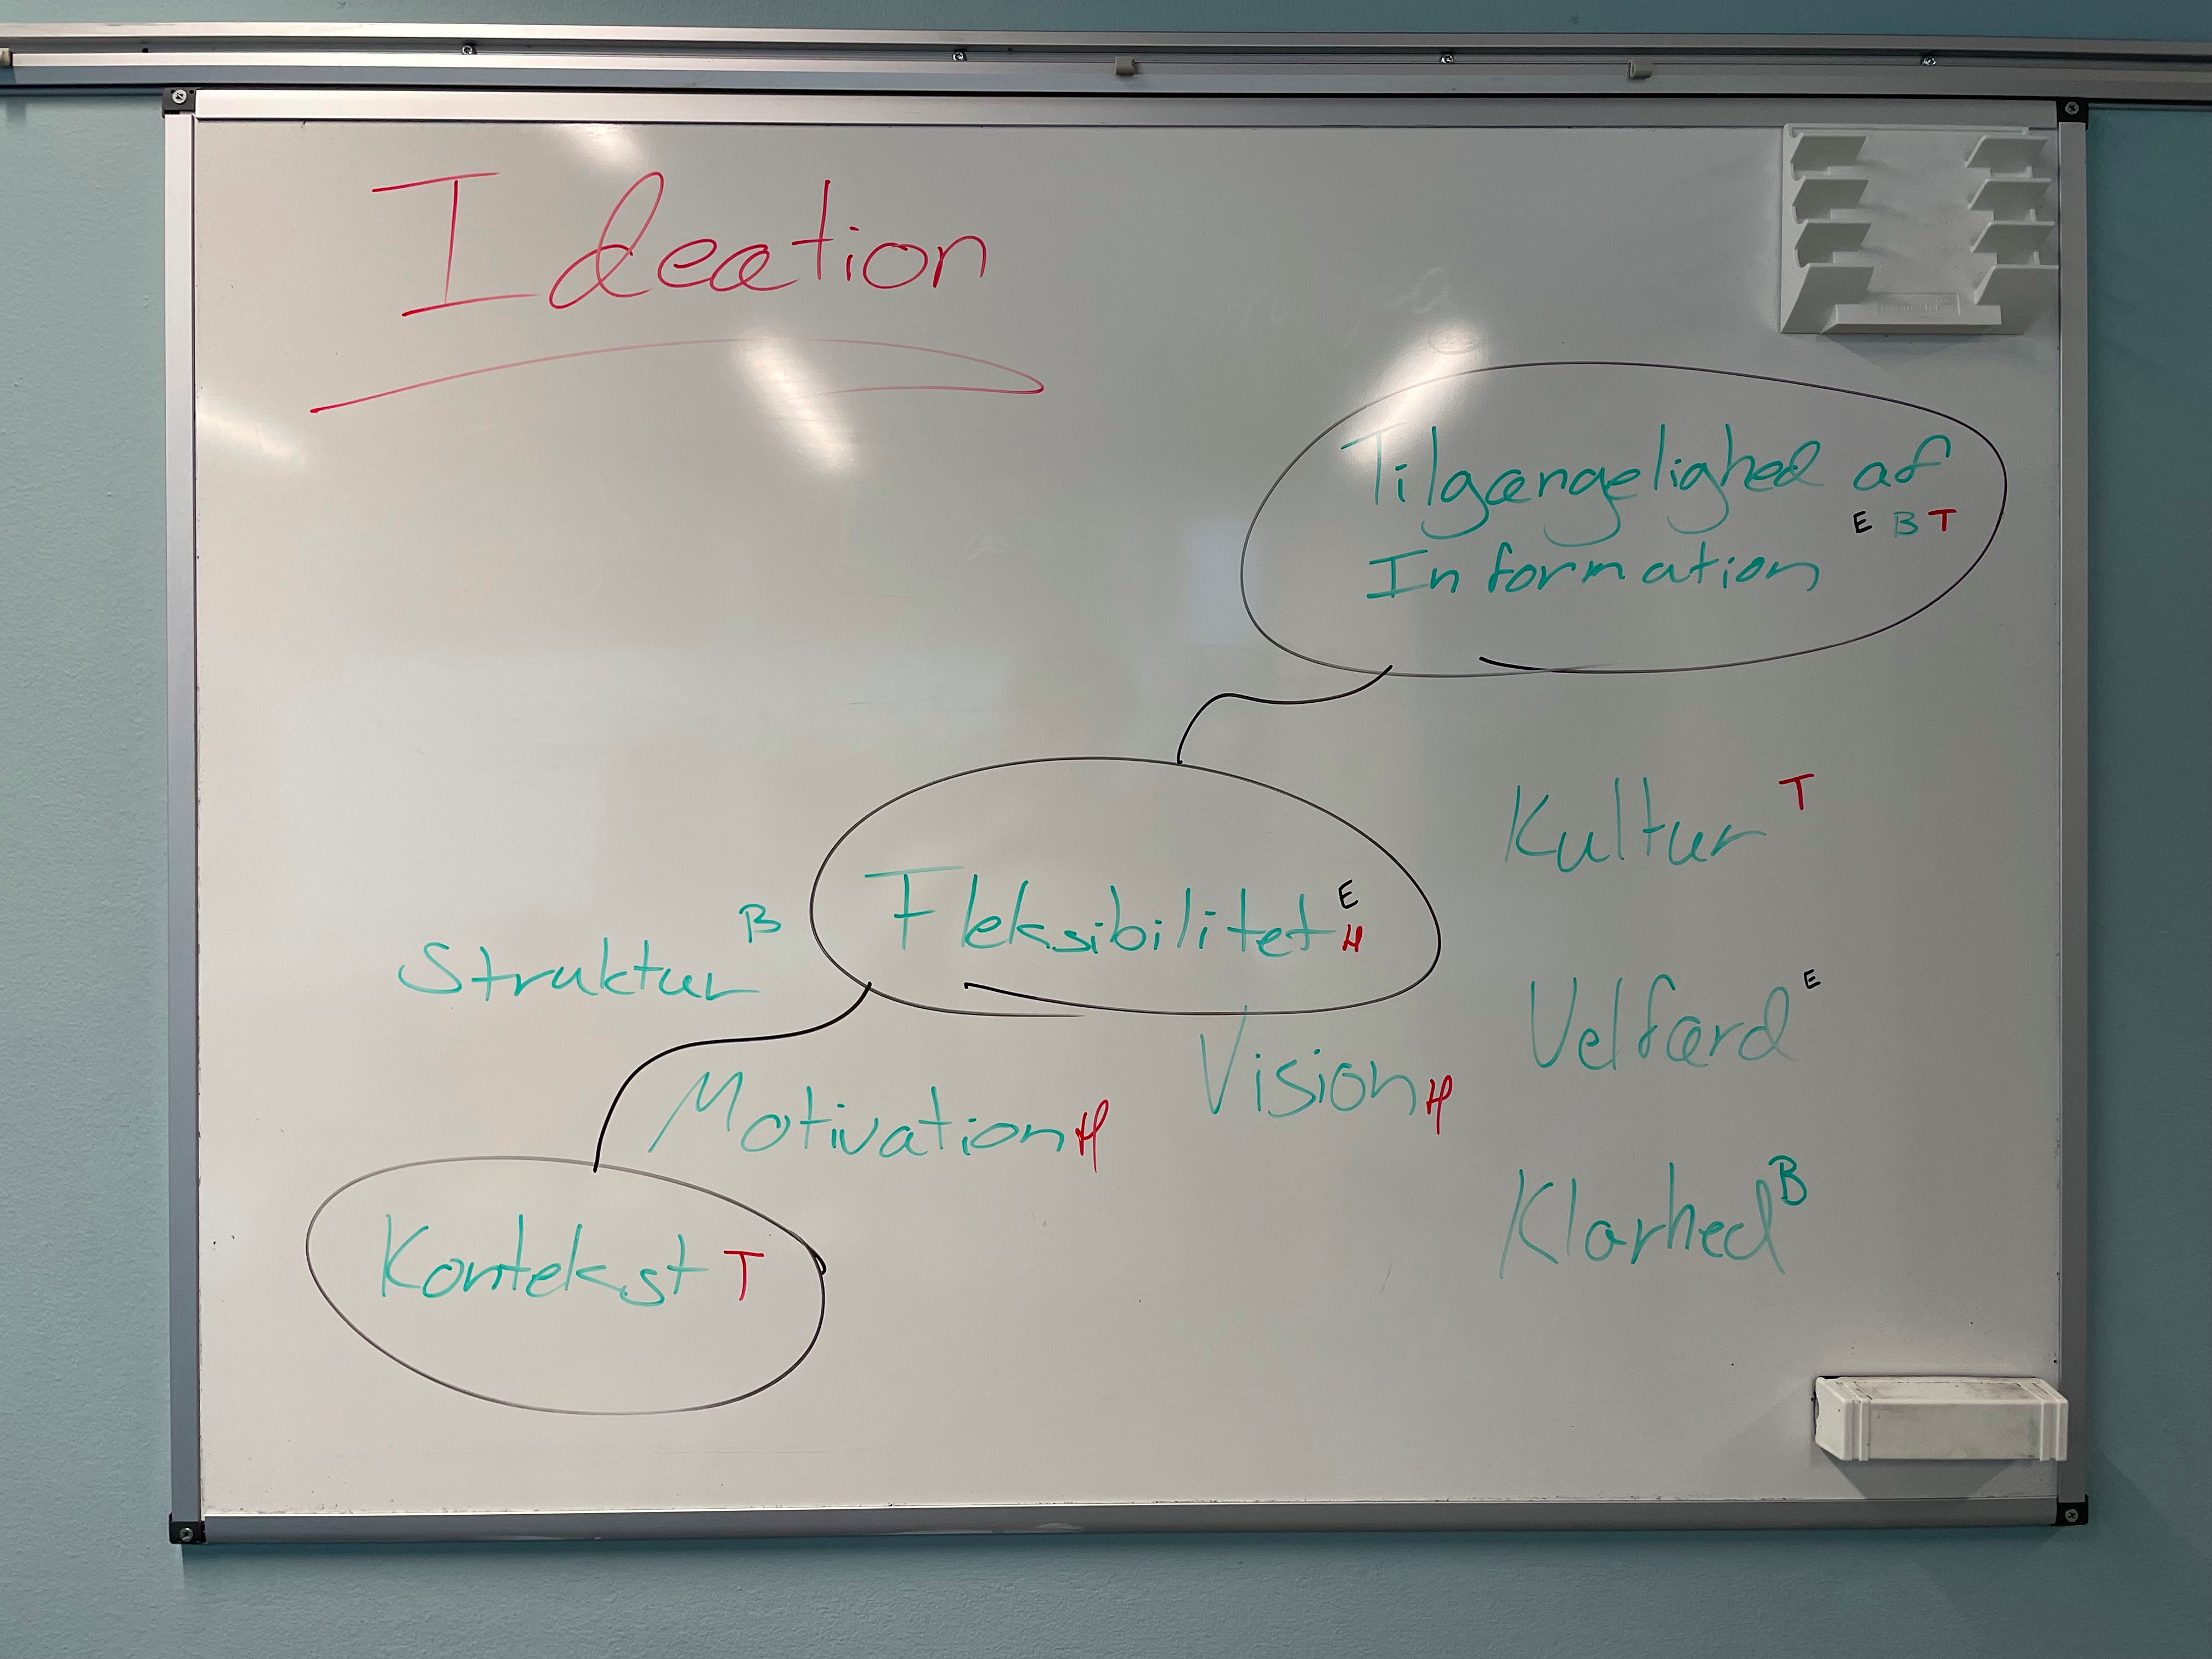
\includegraphics[width=0.32\textwidth,height=\textheight]{./figures/brainstorm_image3.jpg}

\textbf{END images of brainstorming}

Sketches\ldots{} (THOR)

\textbf{START images of sketching}

\begin{pandoccrossrefsubfigures}

\subfloat[]{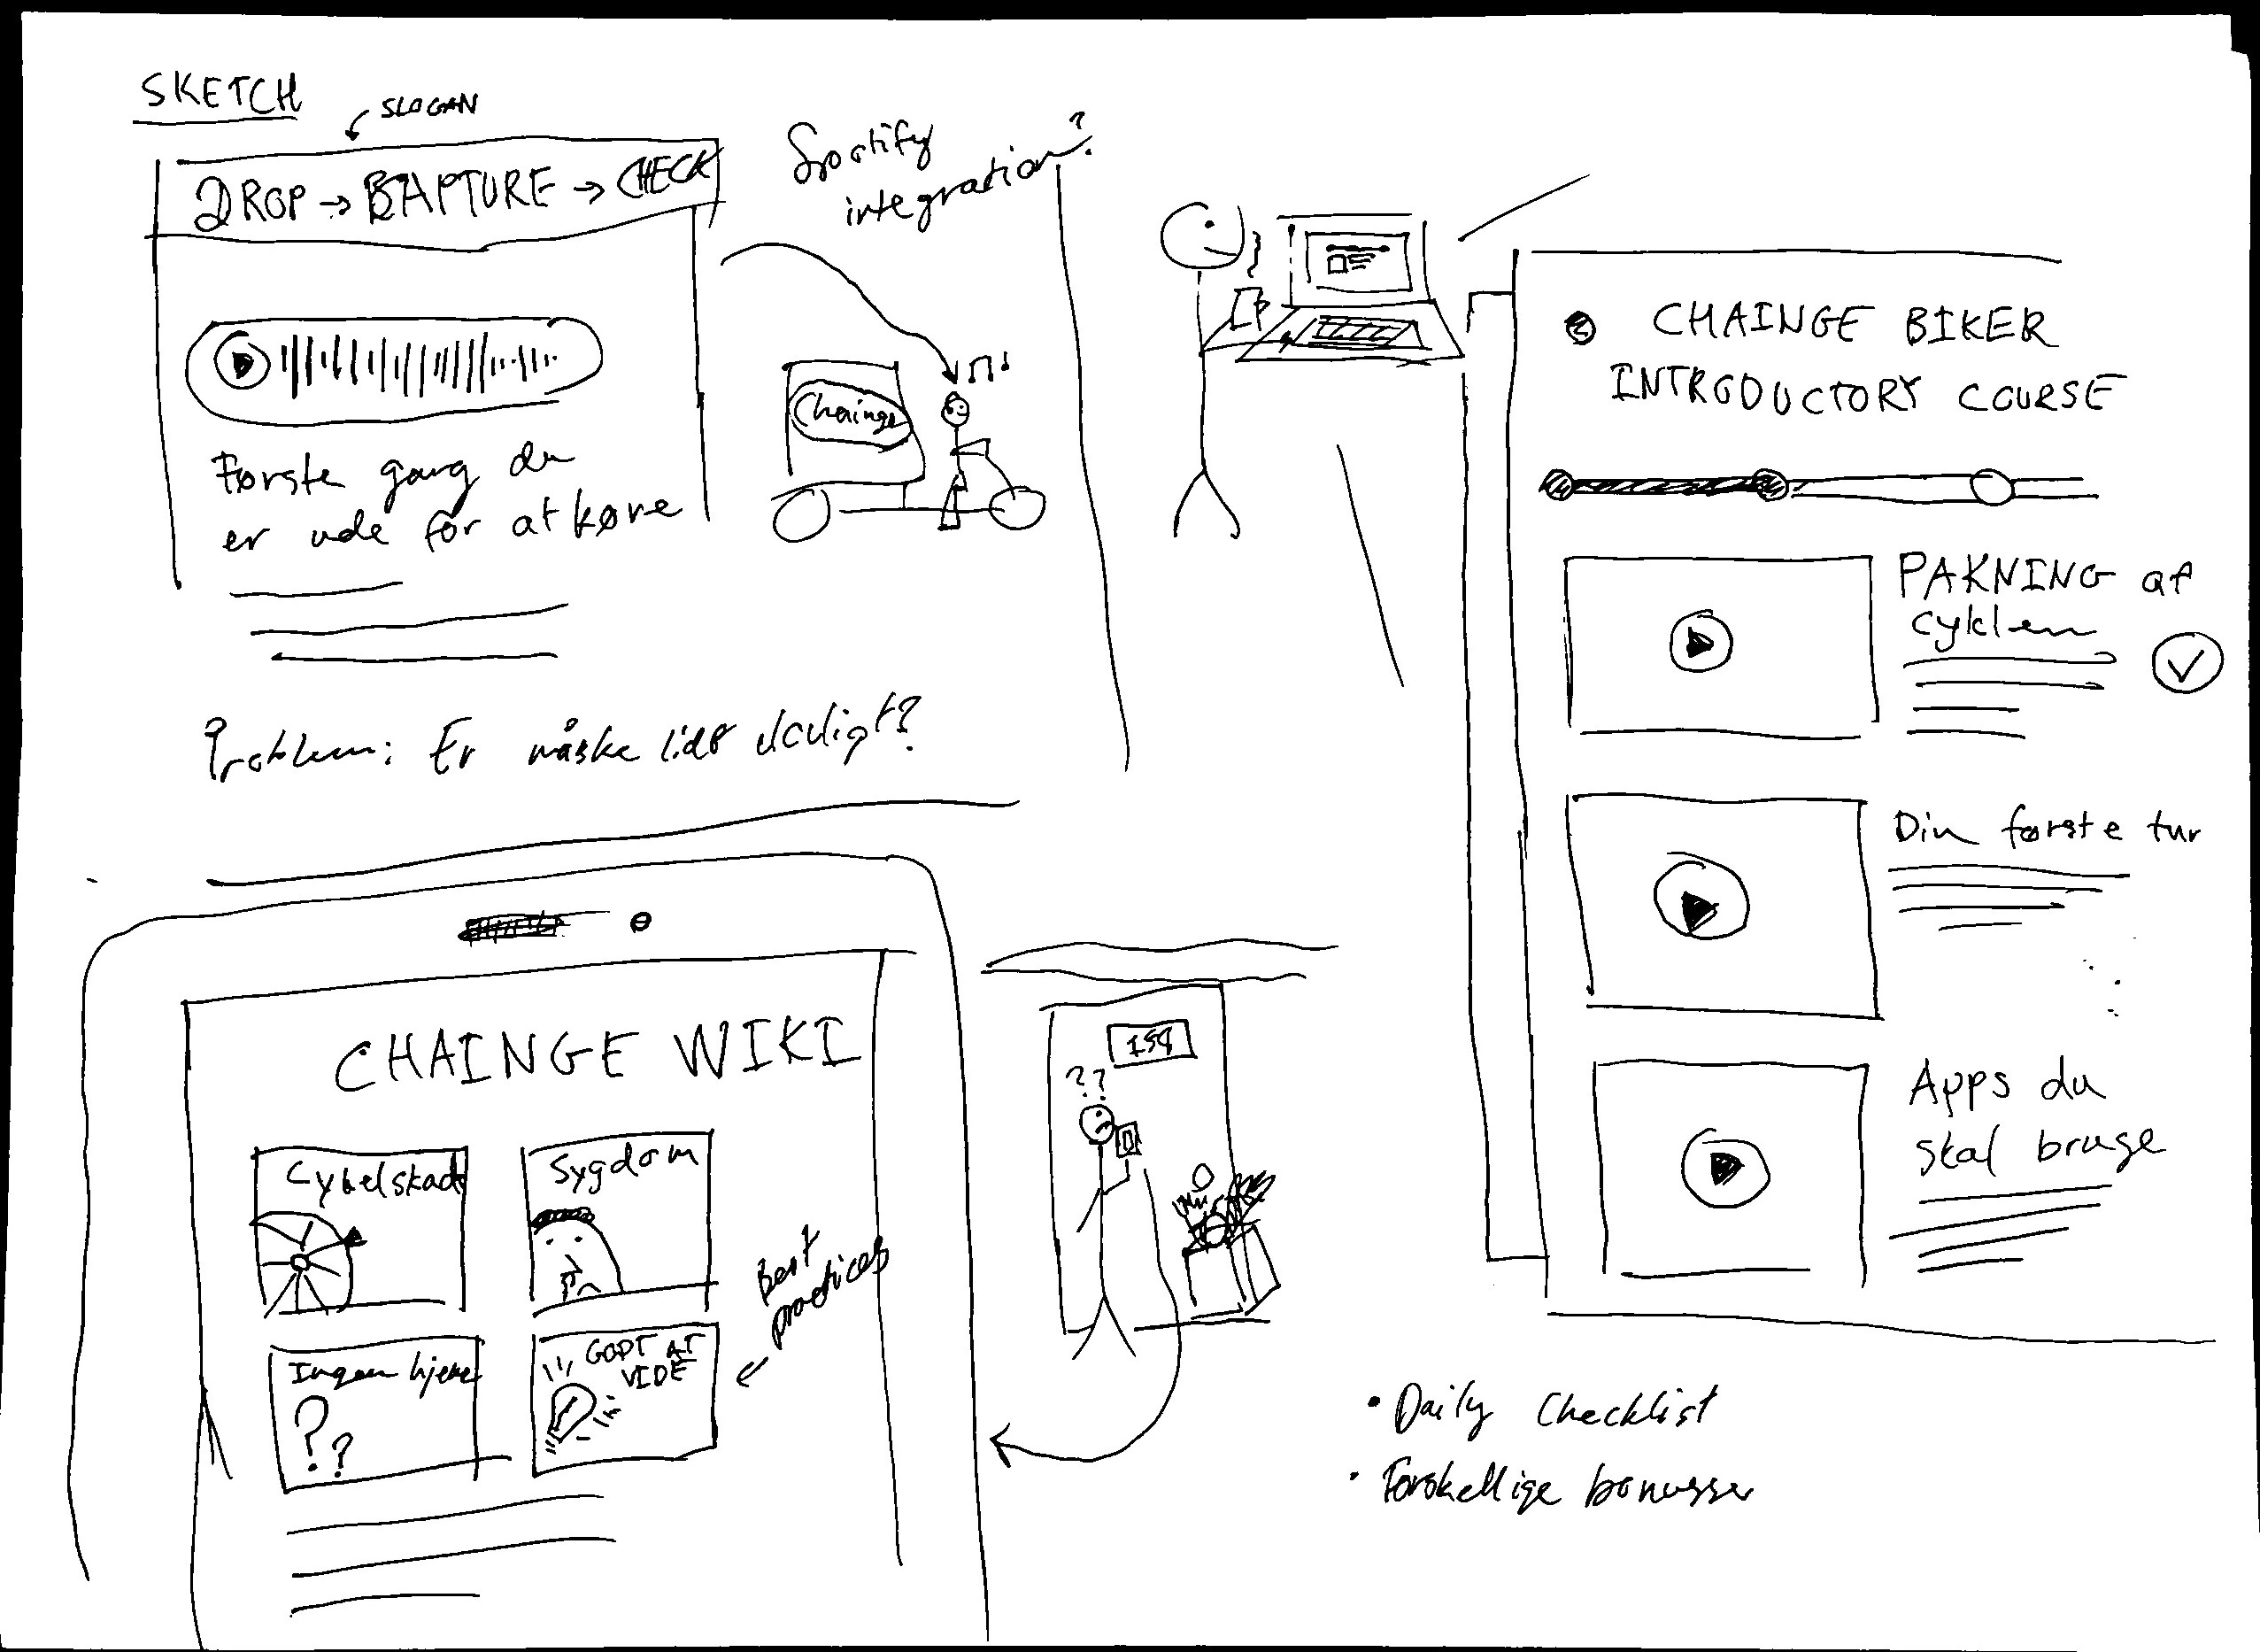
\includegraphics[width=0.49\textwidth,height=\textheight]{./figures/sketching_image1.jpg}}\hfill
\subfloat[]{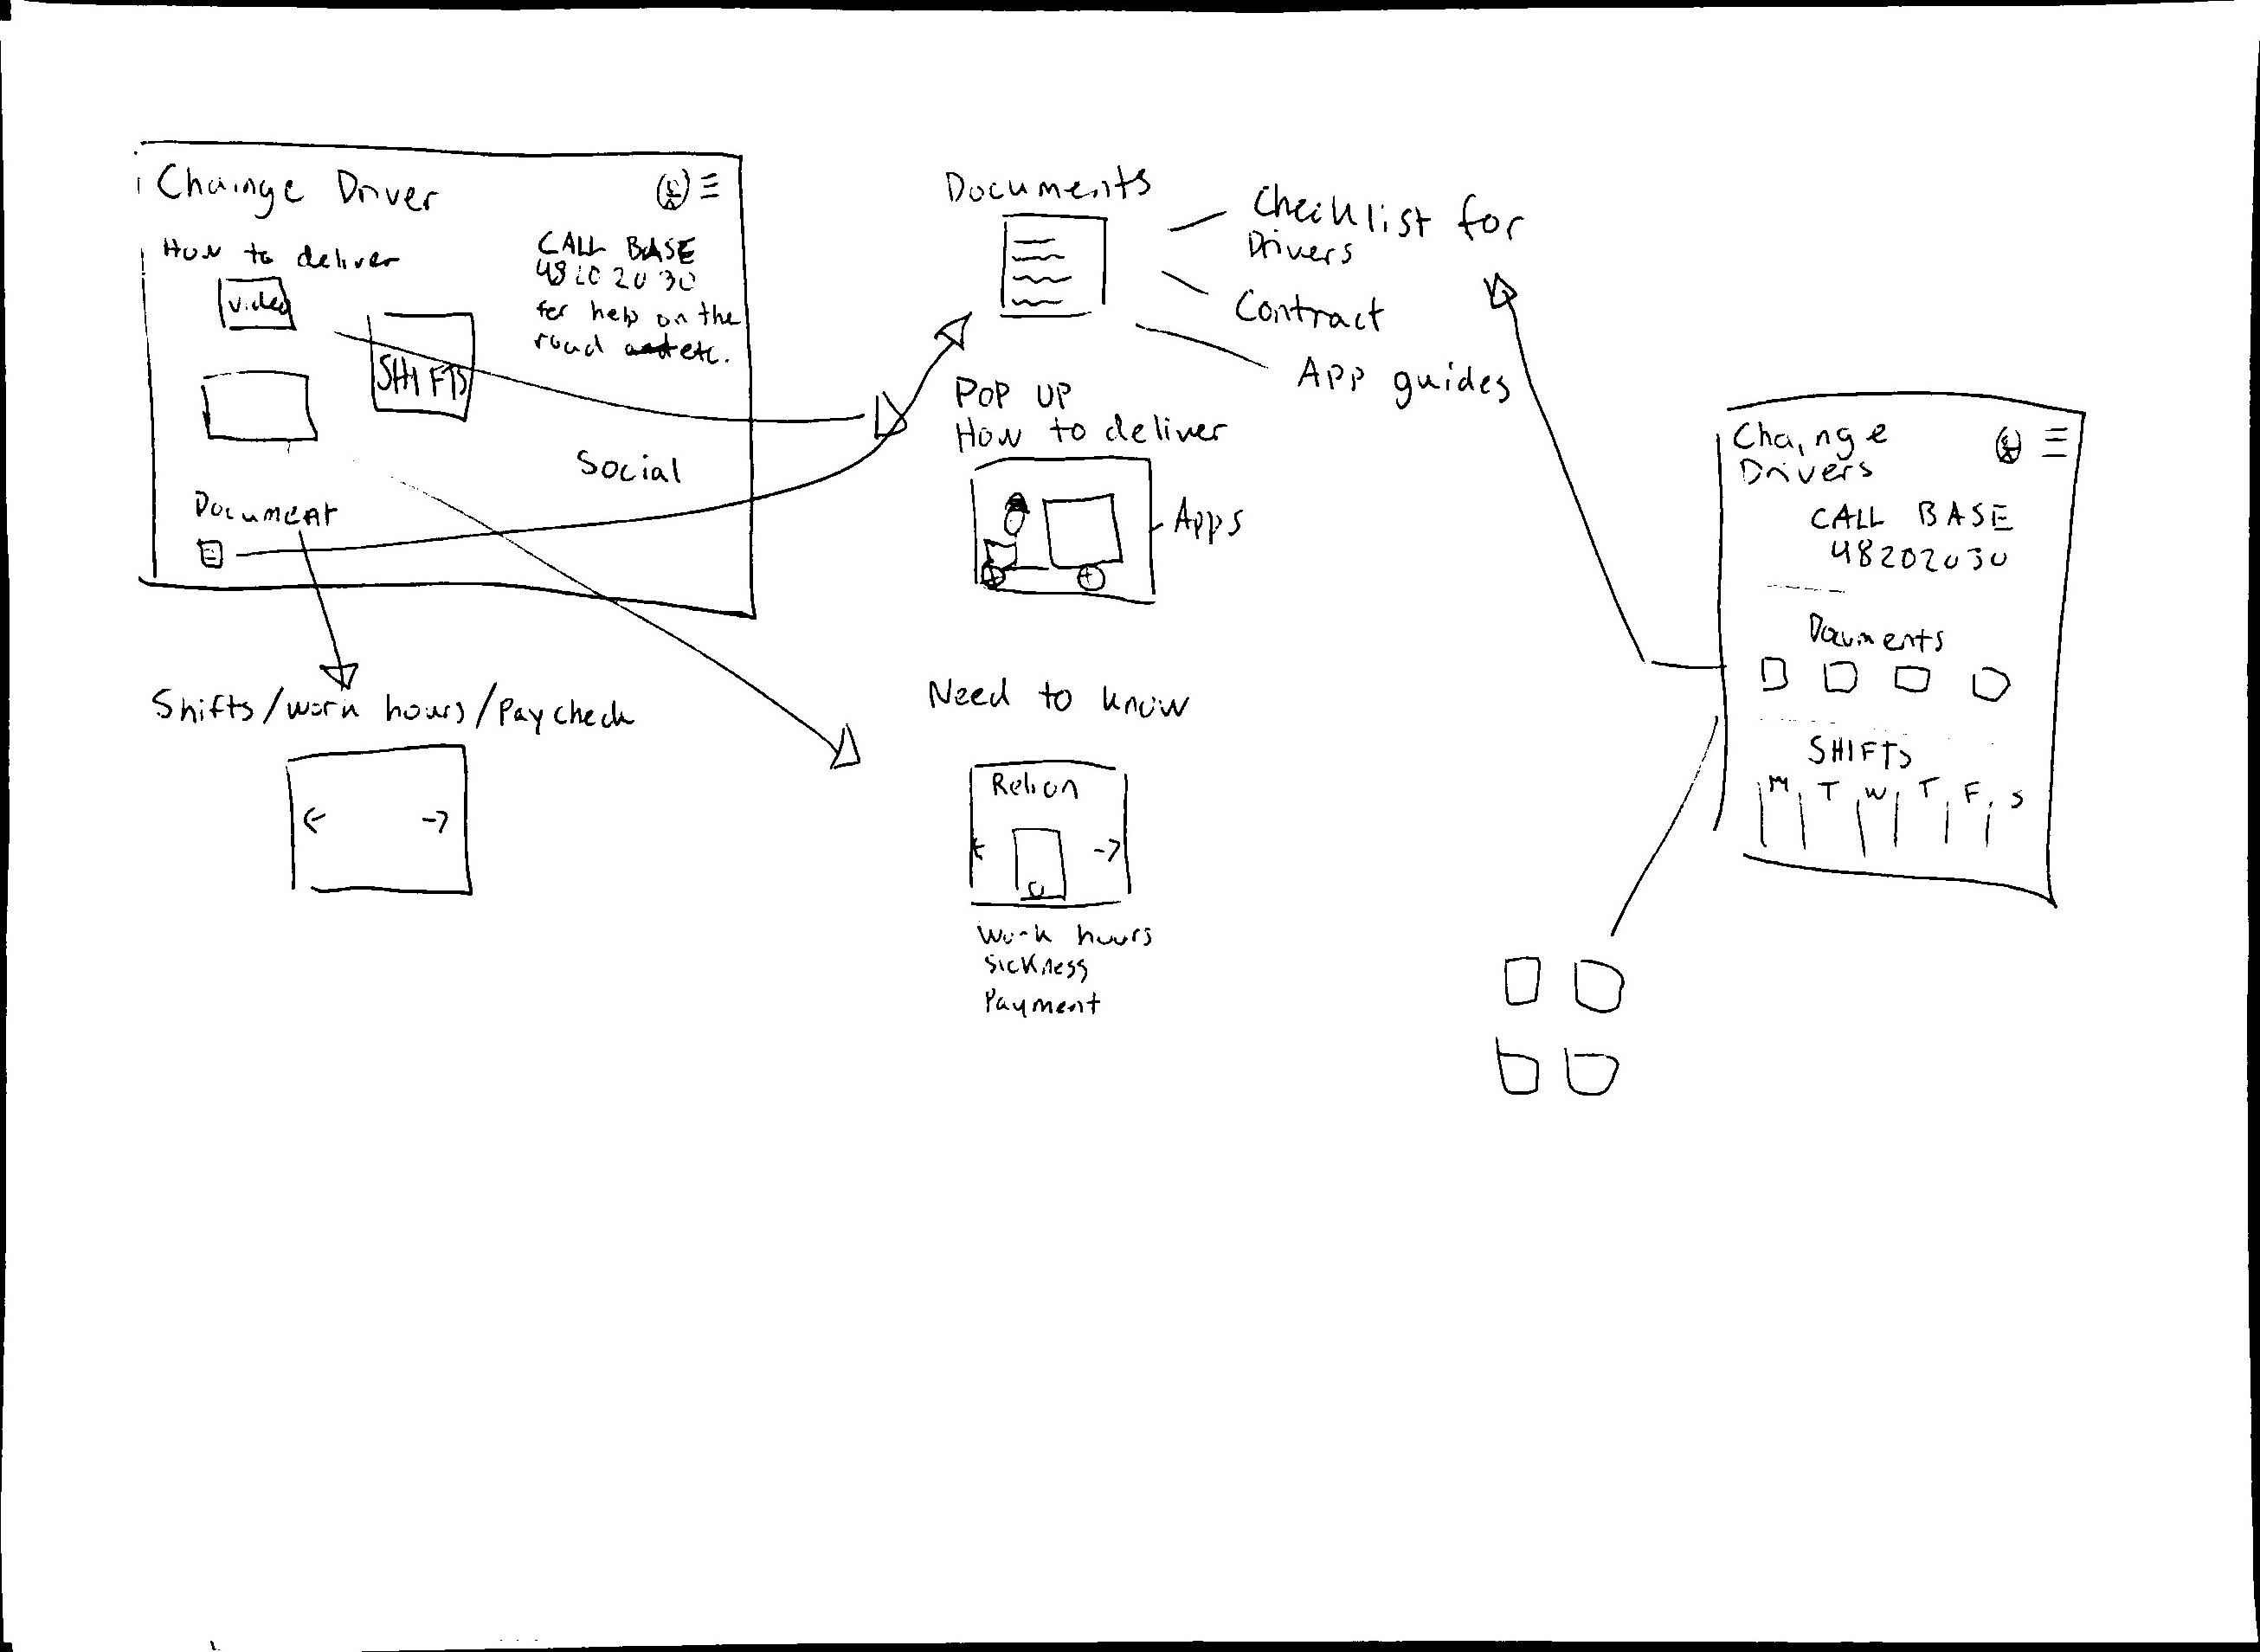
\includegraphics[width=0.49\textwidth,height=\textheight]{./figures/sketching_image2.jpg}}\hfill
\subfloat[]{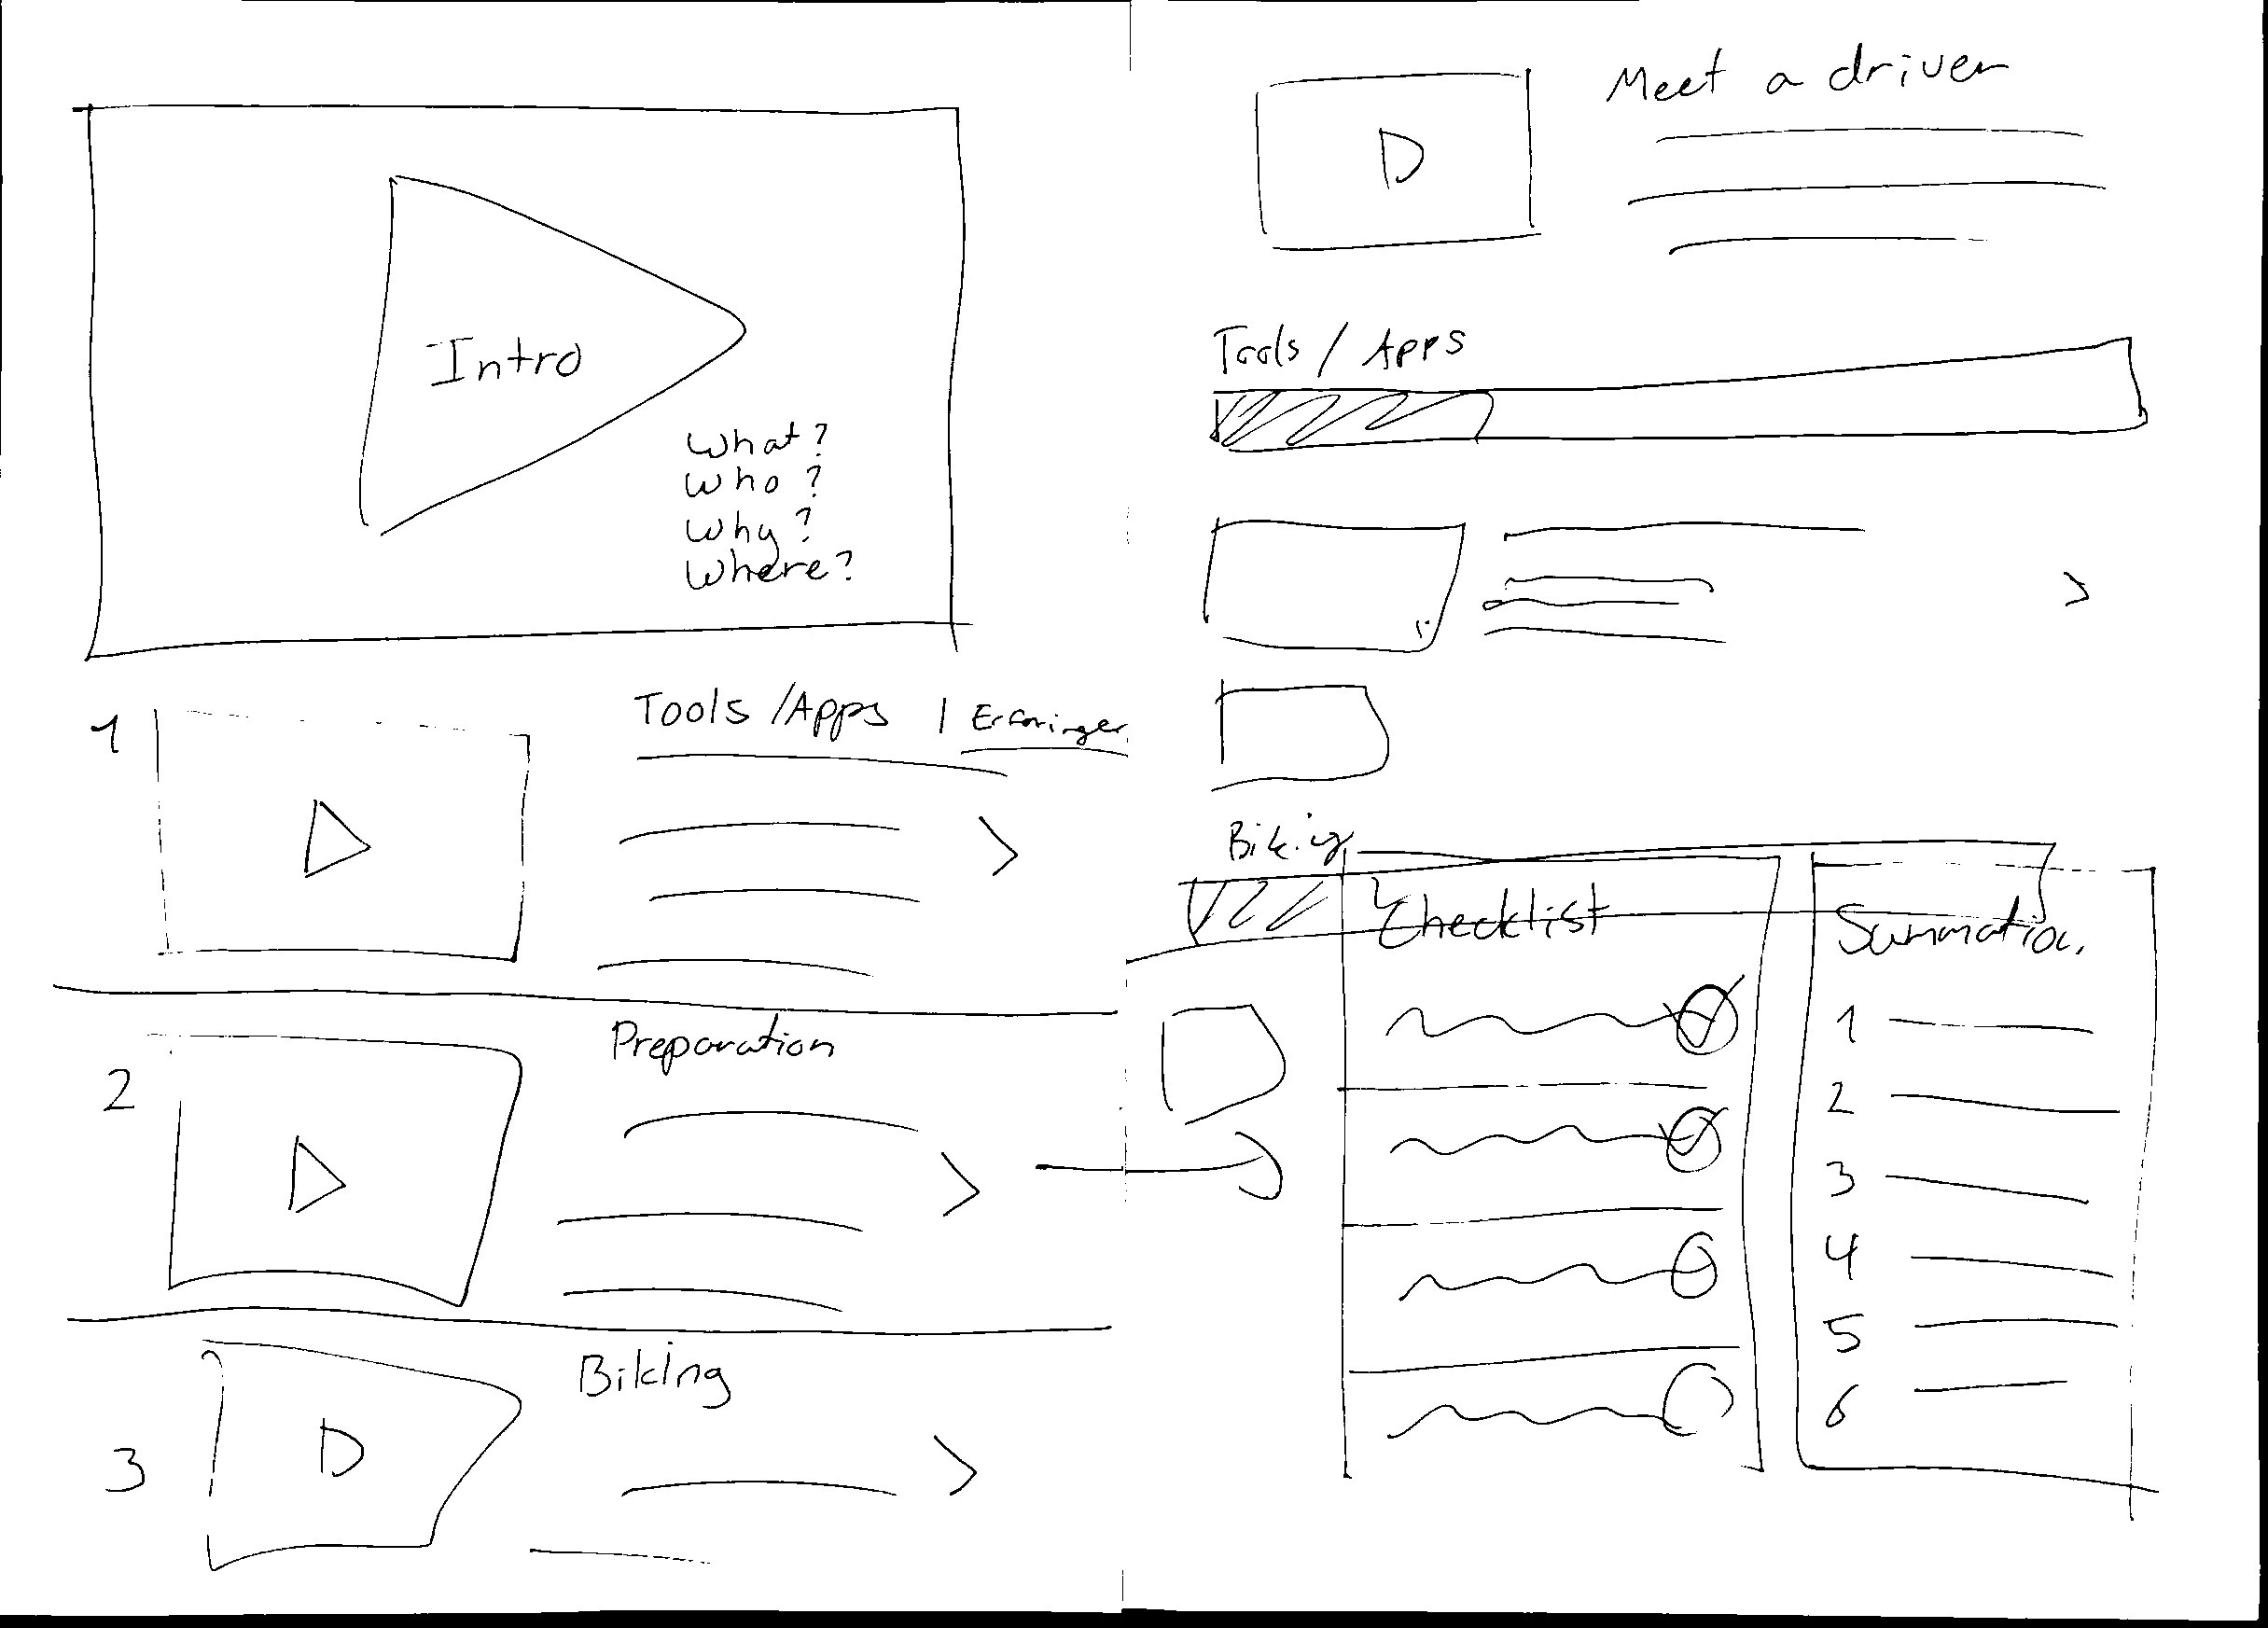
\includegraphics[width=0.49\textwidth,height=\textheight]{./figures/sketching_image3.jpg}}\hfill
\subfloat[]{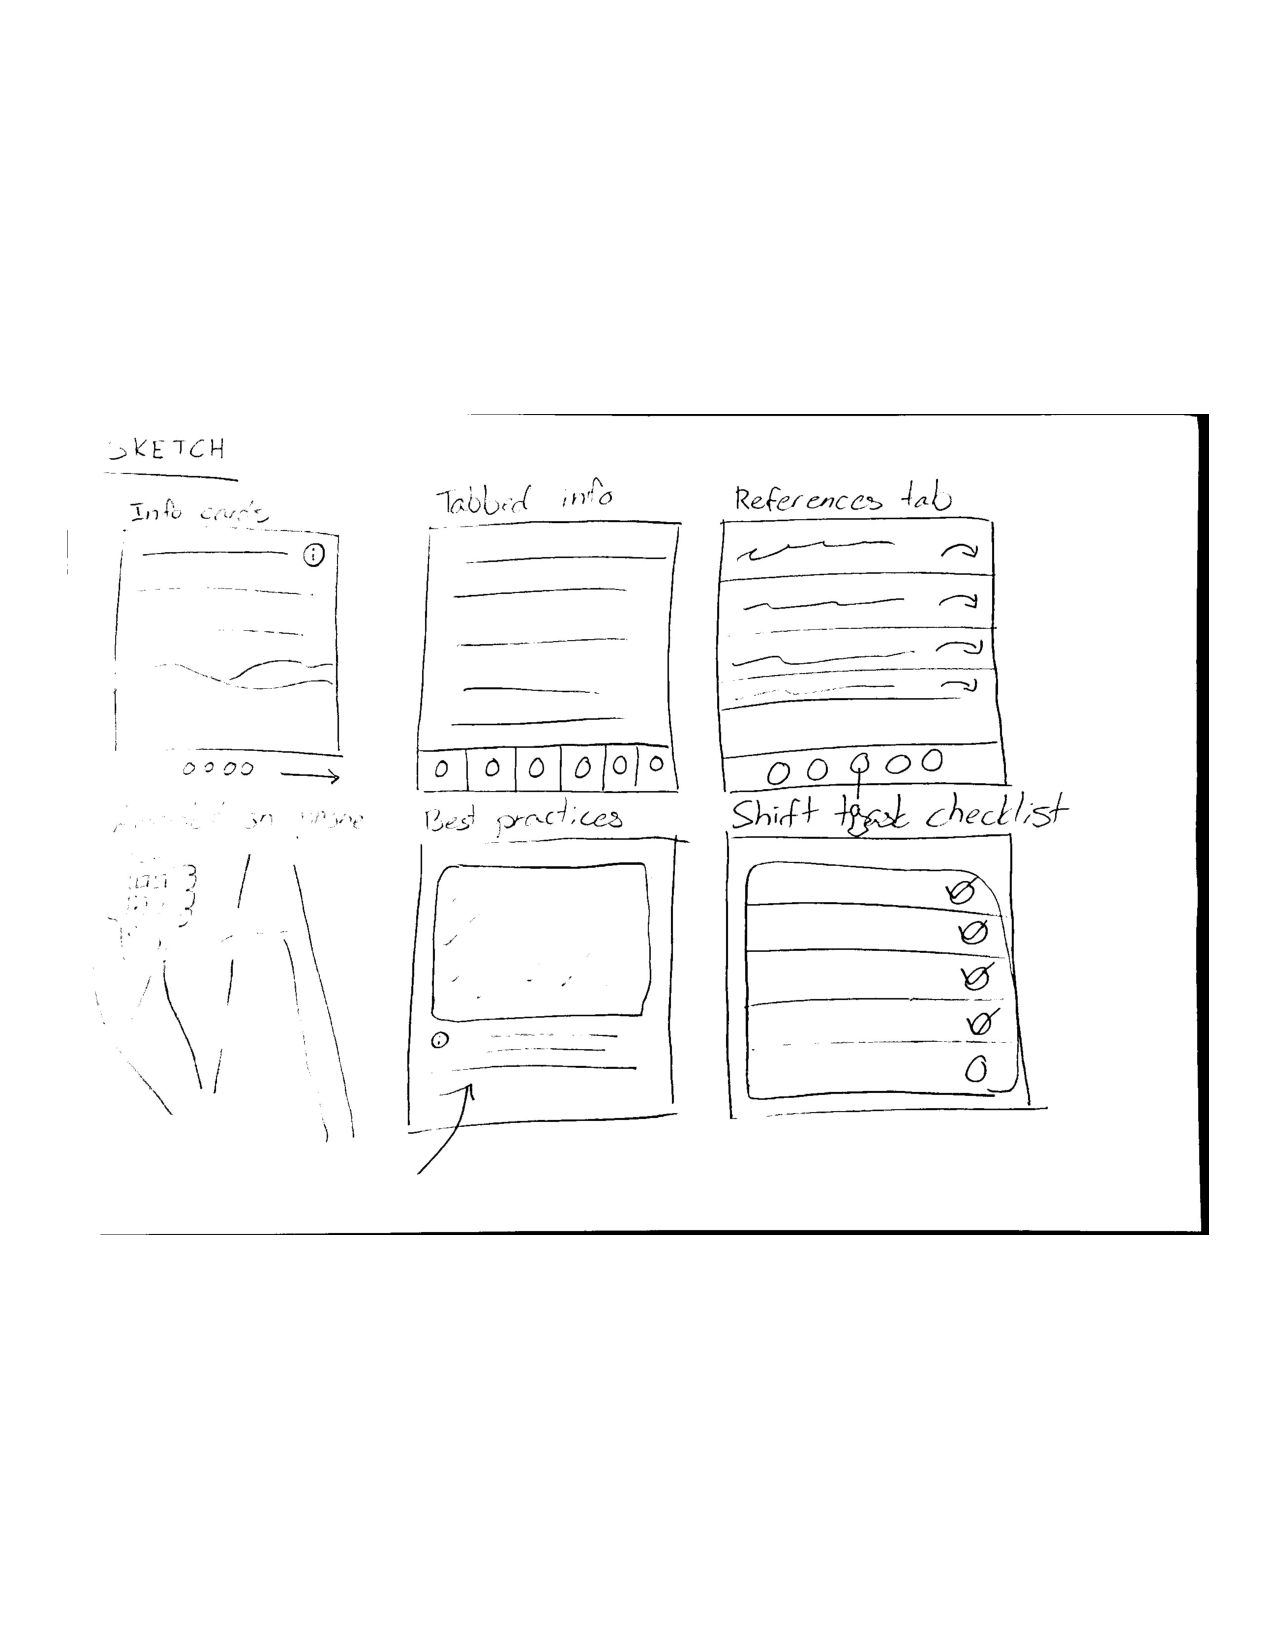
\includegraphics[width=0.49\textwidth,height=\textheight]{./figures/sketching_image4.jpg}}

\caption[{Subfigures caption}]{Subfigures caption}

\label{fig:sketching}

\end{pandoccrossrefsubfigures}

\textbf{END images of sketching}

\hypertarget{sec:prototyping}{%
\subsection{Prototyping}\label{sec:prototyping}}

Our prototyping process began with a discussion of which elements of the
design should be emphasized or de-emphasized. Because our prototype was
a small component in the larger context of a platform, the operational
medium had to be perceivable as one component of many collective
components. We understood this process as experimental development based
on our ideation, \textbf{for the purpose of affirming or denying
preconceived notions}.

Bucheanau and Suri raise the notion that a prototype is any medium
produced to communicate or explore ideas (Bucheanau et al.~2000). Our
goal was to not only communicate amongst ourselves a representation of
our collective ideas, but to also communicate to and explore it with
potential end-users.

Stotlerman et al.~argue that prototypes manifest in three dimensions:
medium, resolution, and scope. Our prototype reflects these dimensions
by being consciously shaped as a digital platform, with a high degree of
fidelity, and a scope fixed to the learning component. We chose to build
a high-fidelity prototype based on our low-fidelity sketches, because we
were less interested in co-designing with users, and more interested in
presenting a highly-structured and accessible platform (Lim, Stolterman
\& Tenenberg, 2008).

\textbf{START mock ups}

\begin{figure}
\hypertarget{fig:mockup}{%
\centering
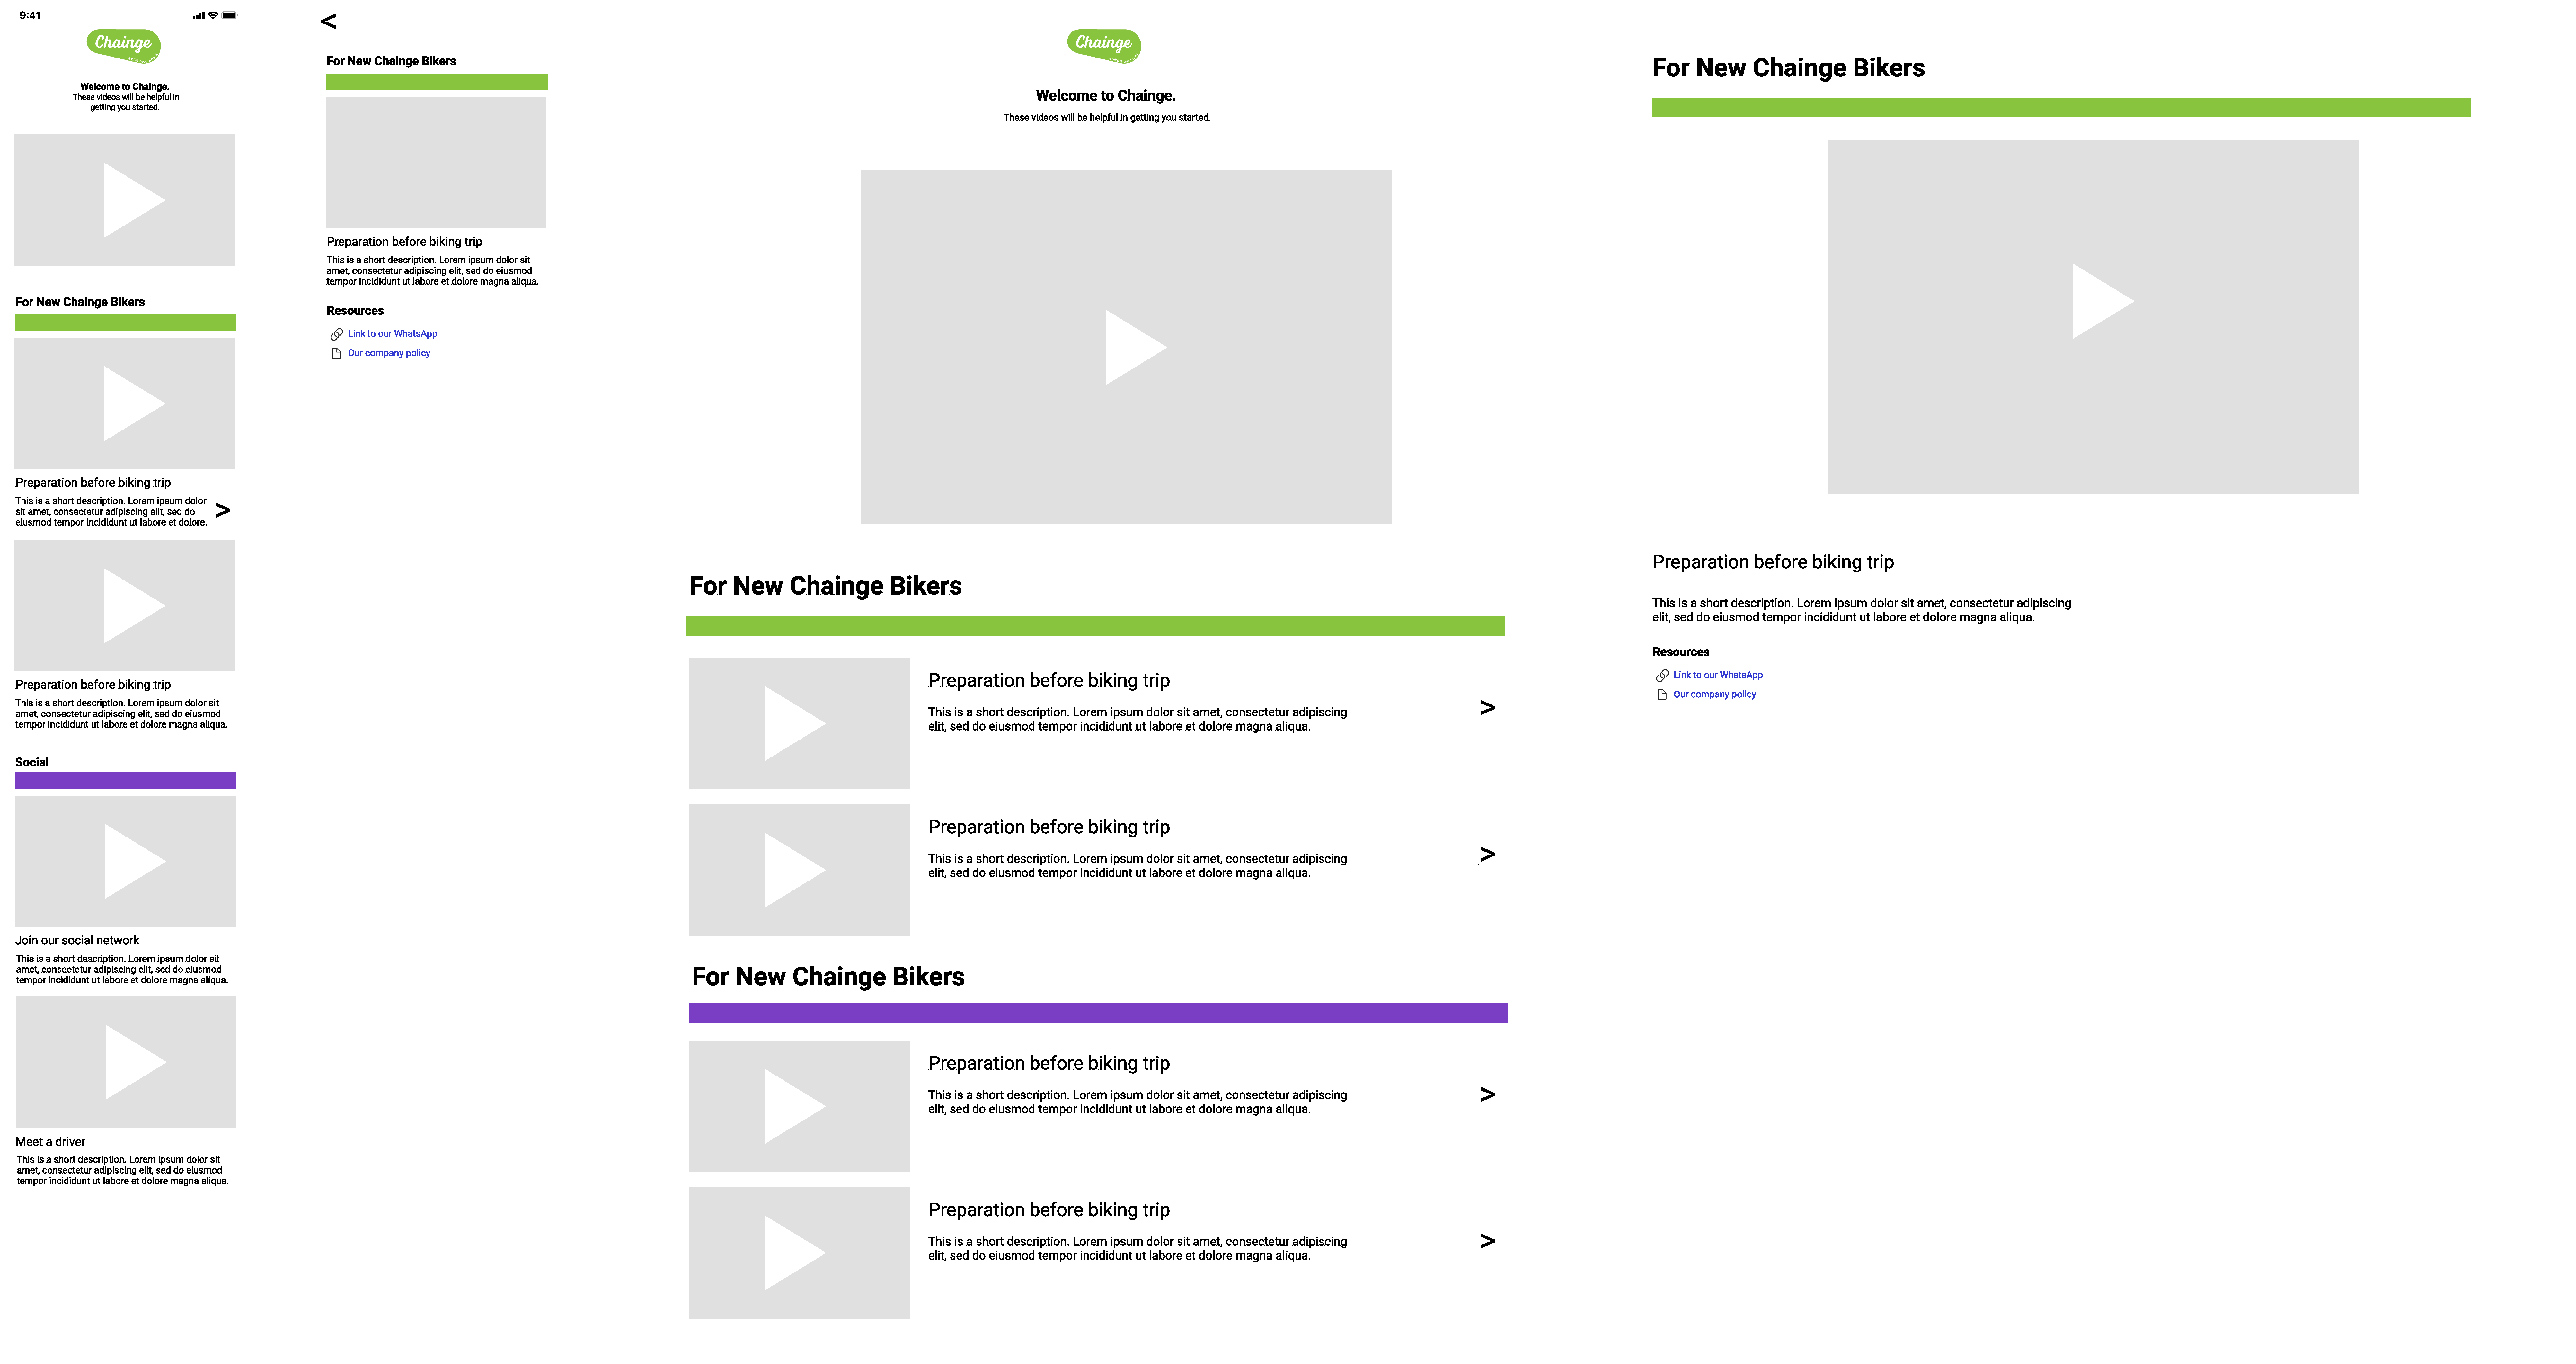
\includegraphics[width=0.75\textwidth,height=\textheight]{./figures/mockup.pdf}
\caption{Mockup of solution}\label{fig:mockup}
}
\end{figure}

\textbf{END mock ups}

\hypertarget{sec:evaluation}{%
\subsection{Evaluation}\label{sec:evaluation}}

We decided to test the prototype with a individual that do not work at
Chainge. The target group of the prototype is new Drivers, therefore we
did not find it relevant to test it on existing employees as they are
potentially biased from their experience working at Chainge. We tested
the platform on a individual studying at ITU. The test was mostly
concerned with a proof of concept and to identify potential pain points.
We wanted to explore if the prototype was easy to navigate.
Additionally, we wanted to show the video on the platform to get
information regarding if it showcases the different work tasks that a
Driver can be presented with.

\hypertarget{sec:findings}{%
\section{Findings (EMIL)}\label{sec:findings}}

Potential Chainge Drivers apply for the job on Chainge's website where
they fill out a formula with their contact information. It is not
required to submit a resume or motivational letter to the application
(Interview 3). The current onboarding process begins with Paul reaching
out to applicants. Paul invites a small group of applicants to visit
Chainge and get an introduction to the job tasks. The interview session
takes around one hour and the applicants are introduced to the
facilities at the headquarter. The applicants try to ride an electric
cargo bike to see if they feel comfortable driving it. One of the
interviewees described the environment during the session as a safe
space as there was no pressure to get on the bike and she experienced a
focus on safety first (Interview 3). The applicants try driving the bike
both with and without the battery to experience the speed (Interview 3).
If the applicants are interested in the job, then a test run is
scheduled a few days later to simulate a typical work day. Afterwards,
the applicants either accept or reject the job proposal (Interview with
Torben).

If the applicants accept, they are given login credentials to various
apps to use when completing work tasks. One of the apps is called Relion
and is used to enter work hours and check planned shifts ahead in time.
There exist different apps to use when delivering packages for the
clients as they all have their individual systems that require a
specific app.

\hypertarget{sec:user_testing}{%
\subsection{User testing}\label{sec:user_testing}}

The testers confirmed that the high fidelity prototype was easy to use.
We wanted to test if the tester understood the Driver's potential work
tasks by viewing the video that we have created. The video is the first
encounter when using the platform. The results of the user testing can
be seen in appendix .

\hypertarget{sec:solution}{%
\section{Solution}\label{sec:solution}}

Due to the scope of the project, the proposed solution is designed for
internal use only as the users are employed at Chainge. The users of the
solution are the new Drivers, existing Drivers and the management of
Chainge. Based on insights from our empirical gathering, \textbf{we
found that some of the Drivers do not speak Danish, therefore we decided
to create the solution in English}. Functionality to change the language
could be added later on to accommodate multiple languages but it was not
prioritised in the prototype.

We have named the solution ``Trainge'' and it consists of a variety of
elements but due to the lenght of the course, we have decided to focus
on the . The developed prototype focuses on an element within the
Trainge platform. The element entails videos to educate new Drivers
about work tasks and tools. When visualising the element, we all had a
similar idea about the design and subconsciously we were inspired by the
Apple Developer app. The inspiration was not intended but it does not
surprise us that we intuitively lean towards the Apple Developer app, as
it is a well known platform for developers.

\textbf{START images of Developer app}

\begin{pandoccrossrefsubfigures}

\subfloat[]{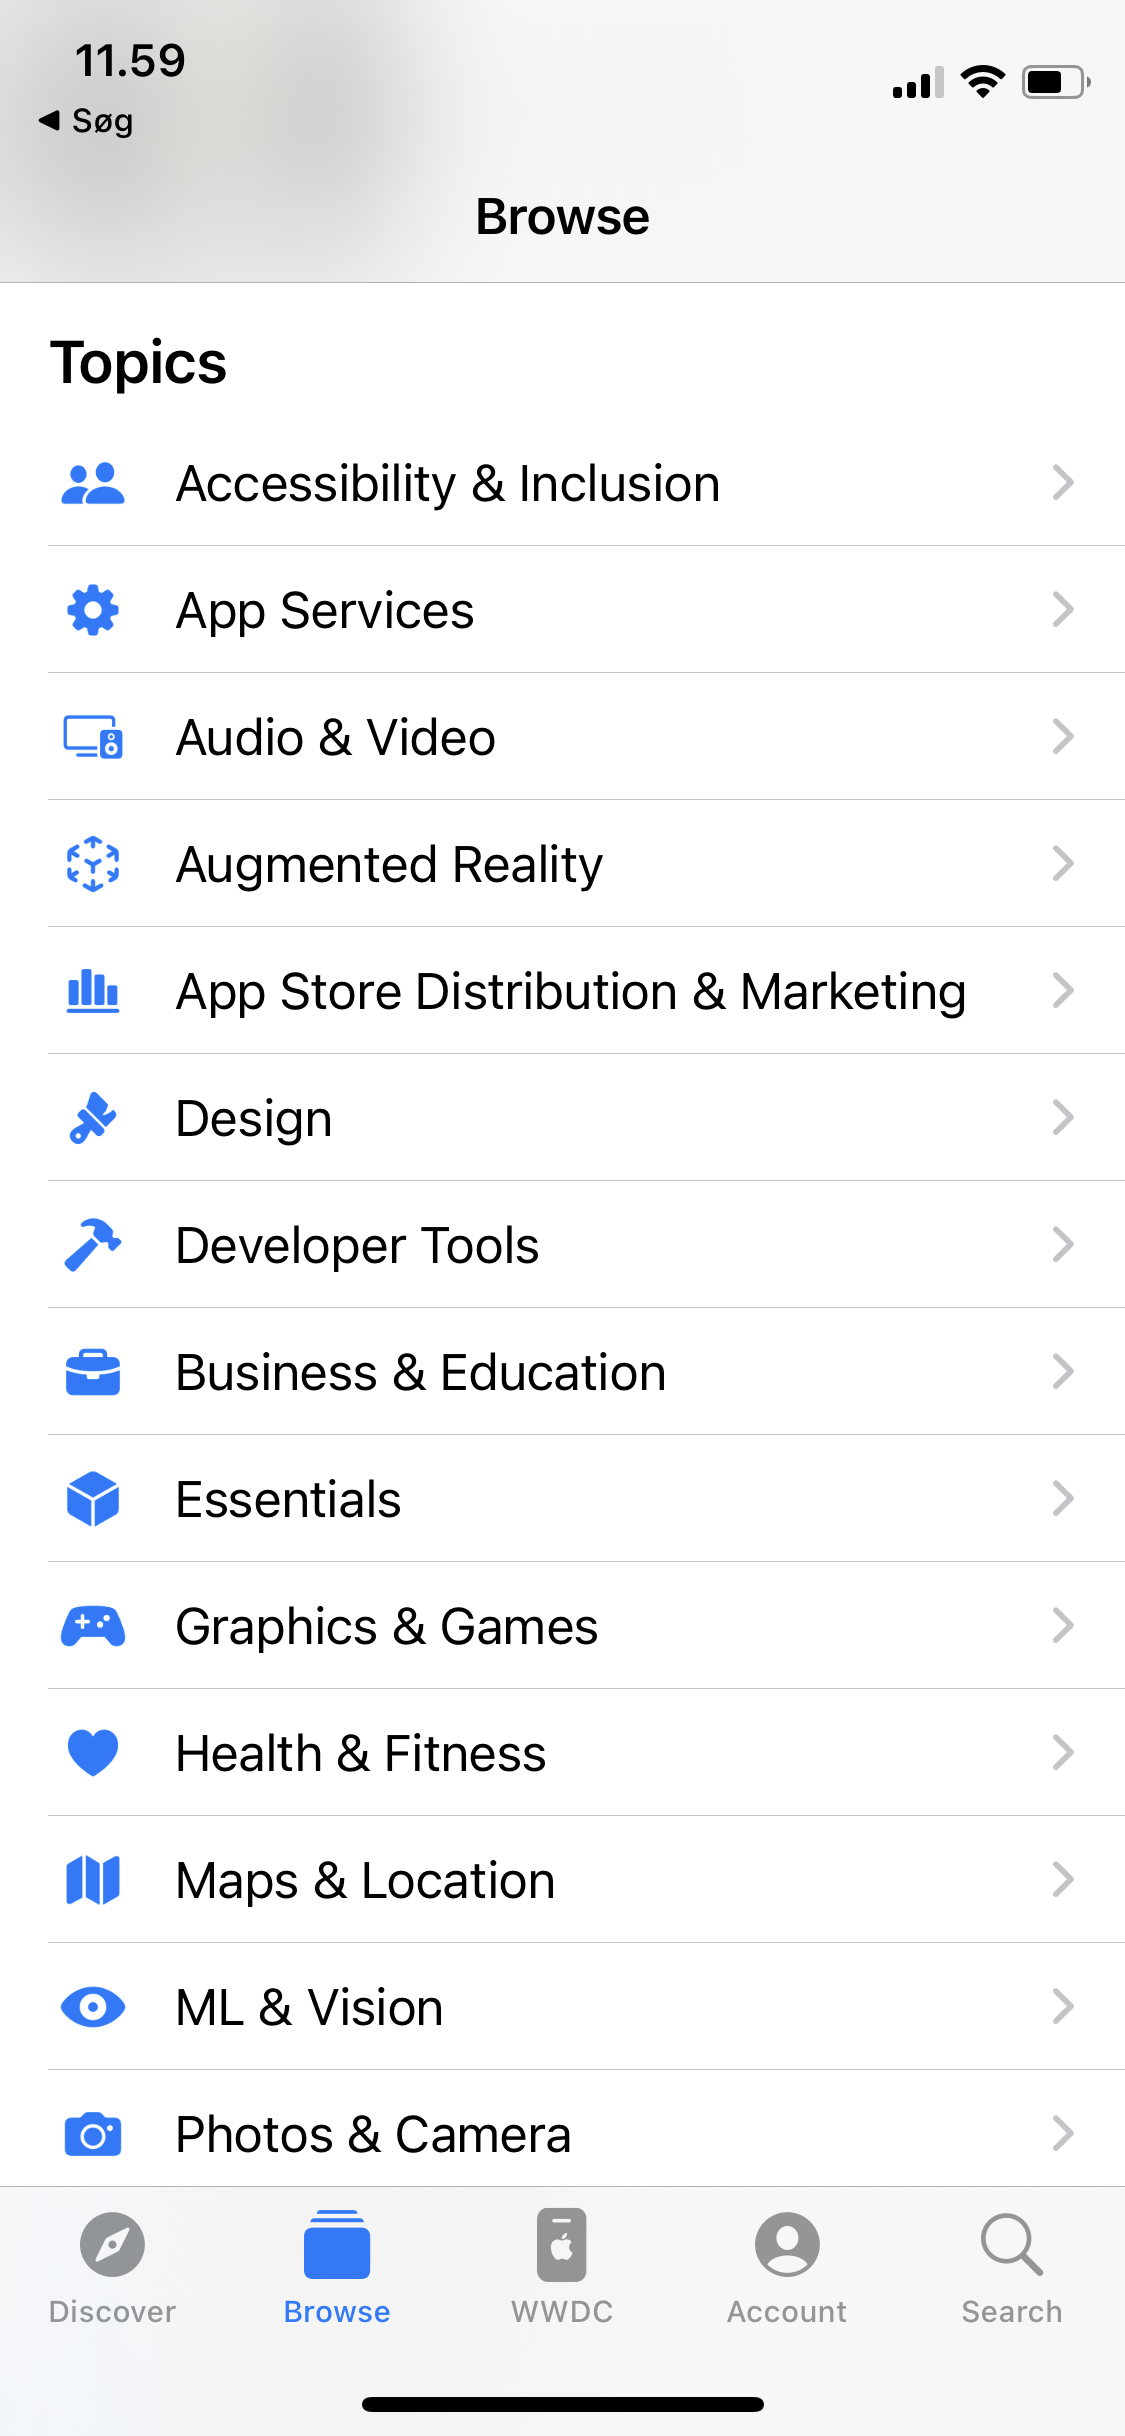
\includegraphics[width=0.24\textwidth,height=\textheight]{./figures/developer_image1.png}}\hfill
\subfloat[]{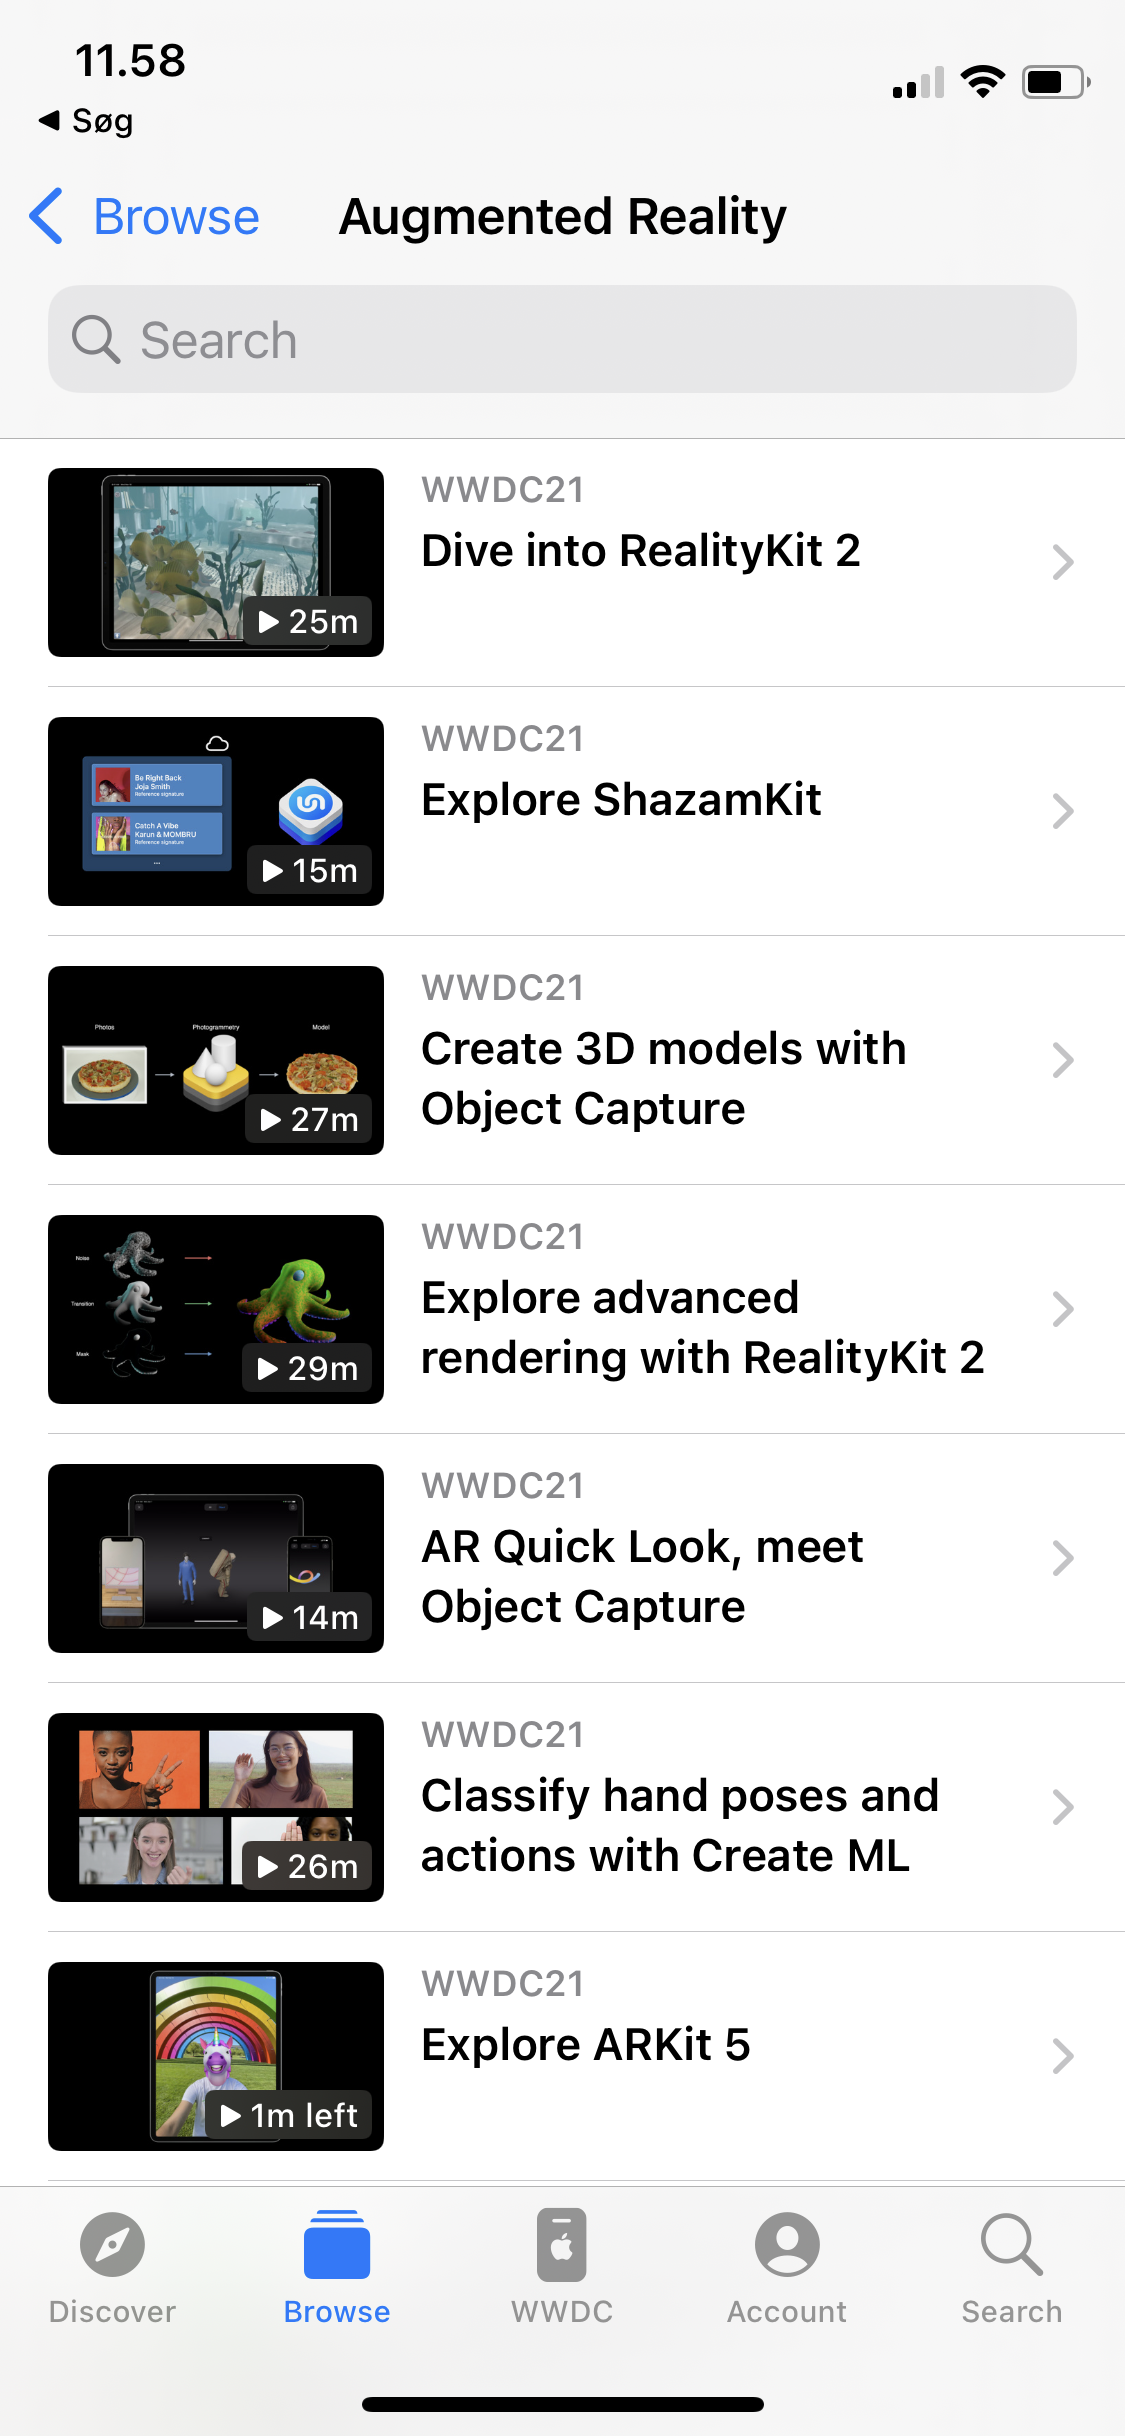
\includegraphics[width=0.24\textwidth,height=\textheight]{./figures/developer_image2.png}}\hfill
\subfloat[]{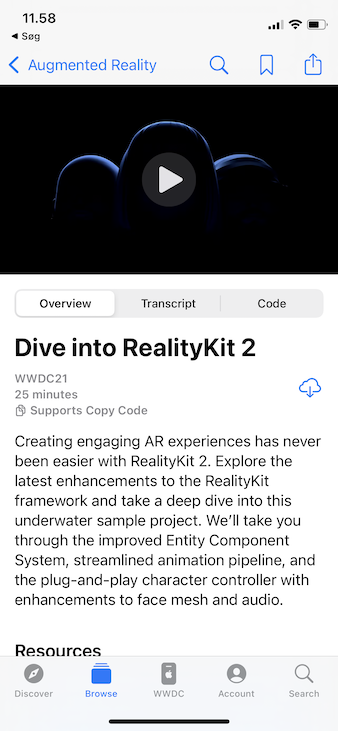
\includegraphics[width=0.24\textwidth,height=\textheight]{./figures/developer_image3.png}}\hfill
\subfloat[]{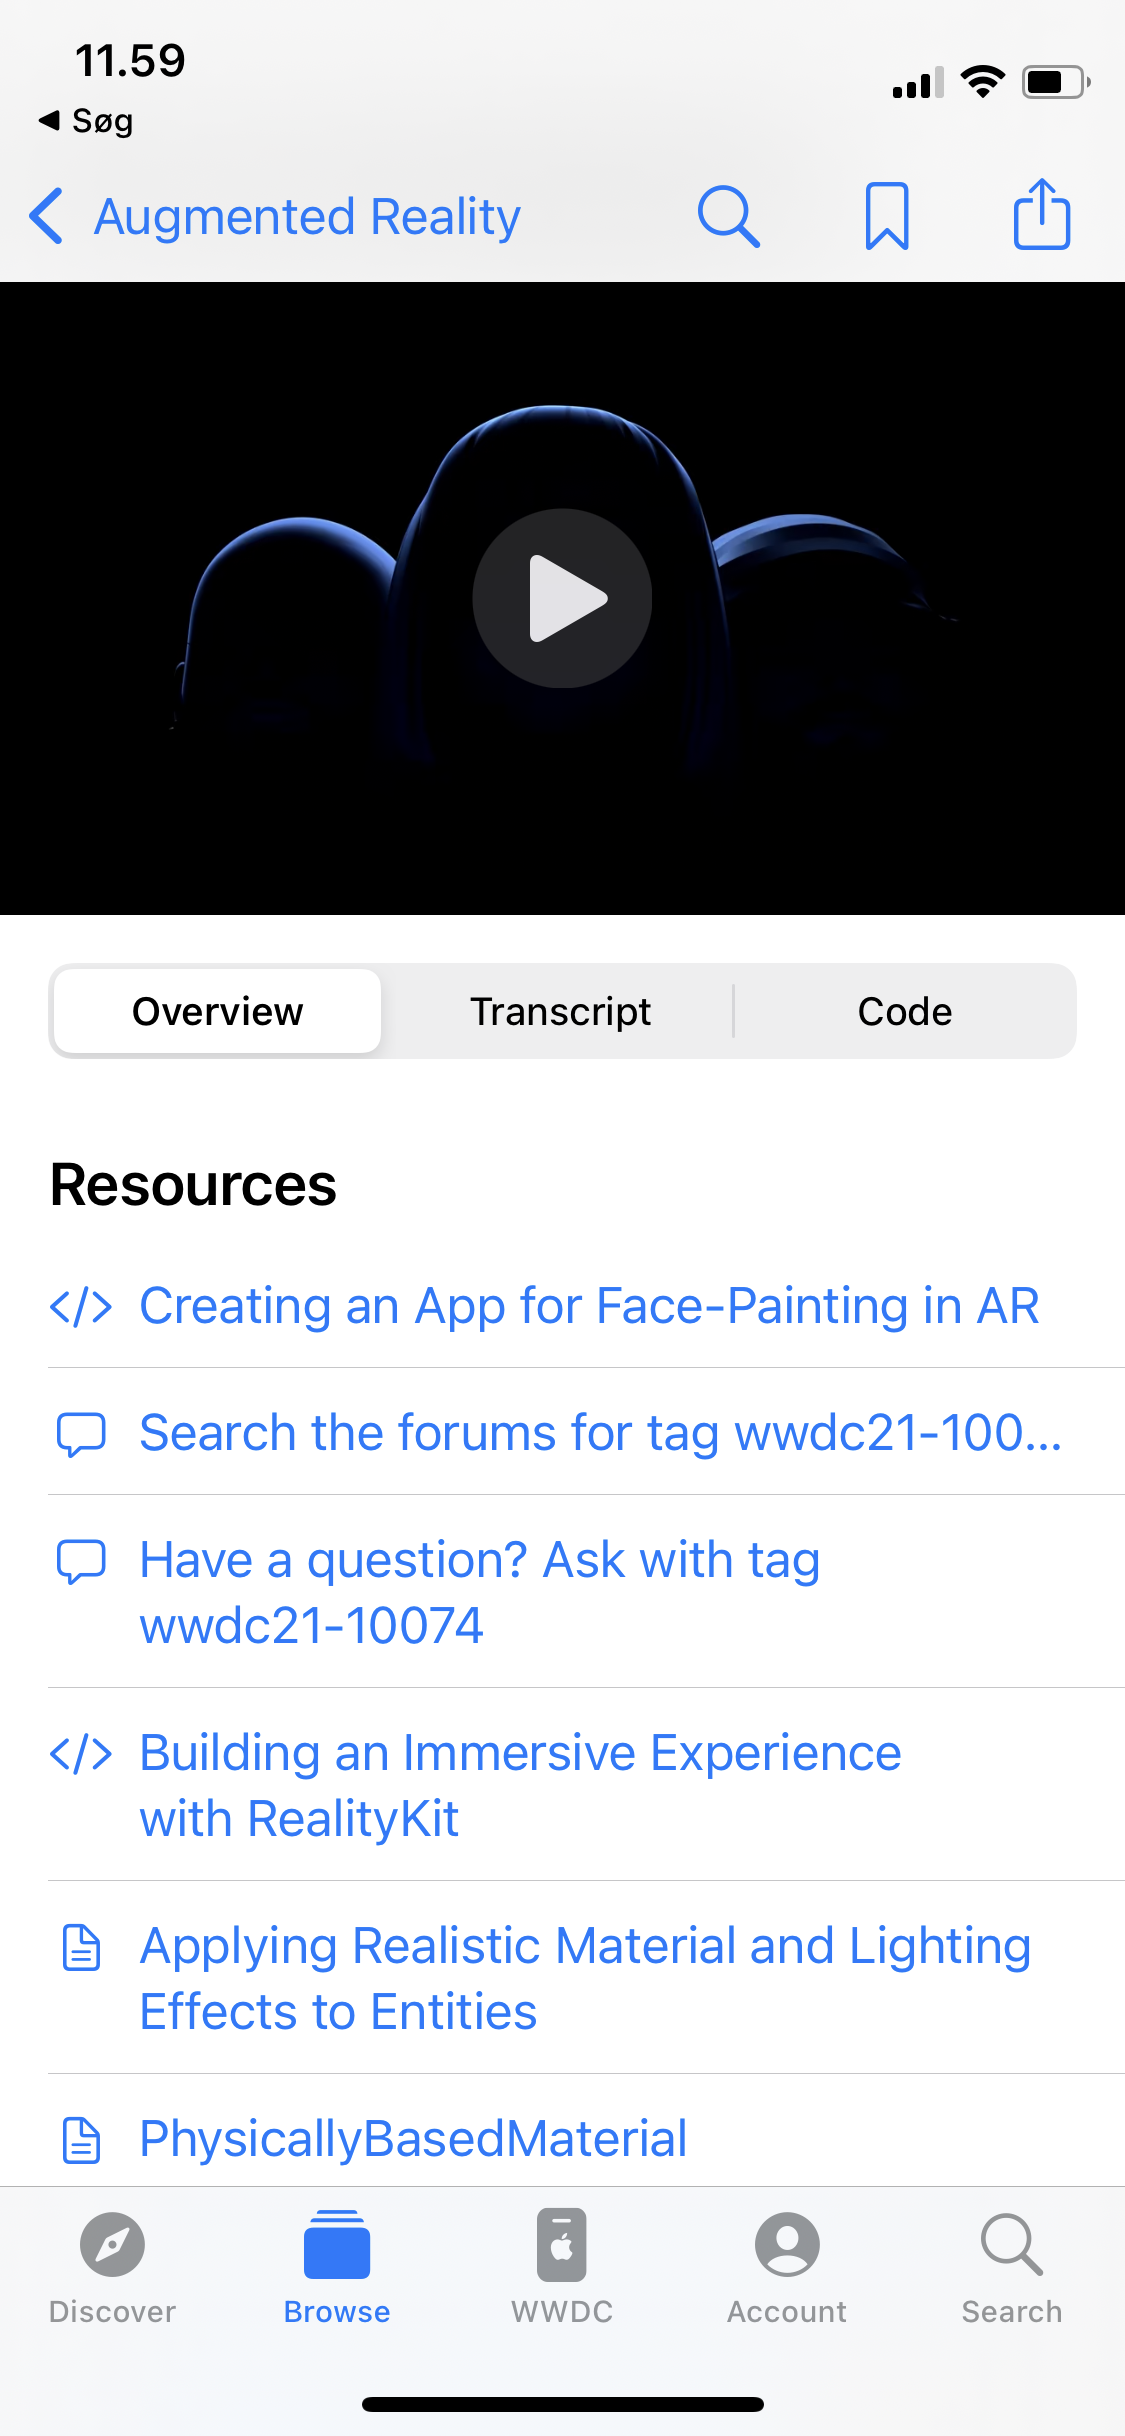
\includegraphics[width=0.24\textwidth,height=\textheight]{./figures/developer_image4.png}}

\caption[{Subfigures caption}]{Subfigures caption}

\label{fig:developer}

\end{pandoccrossrefsubfigures}

\textbf{END images of Developer app}

As stated, the proposed video element is part of a platform that is
accessed with login credentials to personalise the content and to ensure
data security. The idea behind this platform is to create a space for
each individual Driver to obtain and store knowledge relevant to their
job. The proposed solution is designed to assist the Drivers whenever
they need support. For instance, the platform could be useful to utilise
when in doubt of which app to use when delivering packages for a
specific client or how to use internal apps. In this case, the Driver
could watch a video describing in detail what action is needed. One of
the interviewees described that he did not receive an introduction to
how to use one of the apps so he needed to figure it out by himself
(Interview 1). It could be an ideal use case for utilising the proposed
solution to watch a video about the app.

The videos are intended to be informative and function as guidance when
needed. We imagine that the videos are especially valuable in the
beginning of employment when there is a lot of new information and much
to remember.

\hypertarget{sec:organisational_context}{%
\subsection{Organizational context}\label{sec:organisational_context}}

The proposed solution would also be valuable for the management of
Chainge. The platform is digitising and standardising work routines,
consequentially optimising the use of resources spent on onboarding new
drivers. During participatory observation at the headquarters, we
observed a manager at Chainge explaining to three new Drivers how to
pack a cargo bike for a certain client . The manager was also
responsible for picking up the phone if the Drivers were out delivering
packages and needed assistance with situations related to delivering.
The manager's phone rang while he explained the process to the new
Drivers. The resources could be spent differently and the walk-through
could be replaced by a video outlining the process.

The proposed solution could be a valuable asset for Chainge in
allocating responsibilities more efficiently which could have great
impact on the business.

The proposed solution does also entail an element for storage of
documents. The documents should be relevant for the individual employee,
for instance, a work contract and paychecks. The Driver that we
interviewed did not have any knowledge regarding where they could find
their paycheck and one of the interviewees had not received a contract
yet (Interview 1, Interview 2, Interview 3). The described storage
element could be the primary location to place such documents which
would ideally create alignment and eliminate confusion.

\hypertarget{sec:technical_impl}{%
\subsection{Technical Implementation of The
Prototype}\label{sec:technical_impl}}

The Trainge prototype is built as a web application written in a
functional style using F\#, as F\# offers many language features that
prevent program errors compared to other languages such as Javascript or
Typescript. Using the Fable F\# to Javascript compiler, the prototype is
then able to be run as a web application in the browser. The F\# code
robustness is transitively applied to the resulting compiled Javascript
when using Fable.

Several large frameworks are used to realise the prototype, mainly the
React and Bulma frameworks which are used to define the structure, look
and reactivity of the prototype. Reactivity is important, as it allows
the UI to become driven by data instead of imperatively/manually
updating relevant UI components when the underlying data changes. This
is automatically afforded to us using React. As React is not a native
framework to the F\# language, an auxiliary library called Feliz is used
to interface between F\# and the Javascript-based React framework.

The code is structured using the Elm Architecture (TEA). TEA is a way to
split an application into smaller applications or components that are
easily composed together without introducing unnecessary coupling
between said components. Essentially, it is a way to control `spaghetti'
code and make sure that error inducing changes in one part of the
prototype does affect another part of the prototype. This is strictly
not necessary for a small prototype as Trainge, but hugely useful in the
case Chainge needs to scale up the prototype to a fully fledged
application.

\hypertarget{sec:discussion}{%
\section{Discussion}\label{sec:discussion}}

\hypertarget{sec:reflexivity}{%
\section{Reflexivity}\label{sec:reflexivity}}

\begin{itemize}
\tightlist
\item
  Not an iterative approach because the solution is not tested on
  users/non-users (Emma)
\item
  Used double diamond model as 1) we needed to create prototye and 2) we
  needed a common language to understand where we were in the process
  and where we were headed.
\item
  Why did we do what we do
\end{itemize}

\hypertarget{sec:conclusion}{%
\section{Conclusion}\label{sec:conclusion}}

\newpage

\hypertarget{sec:bibliography}{%
\section{Bibliography}\label{sec:bibliography}}

\addvspace{0.5cm}

\hypertarget{refs}{}
\begin{CSLReferences}{1}{0}
\leavevmode\vadjust pre{\hypertarget{ref-bradbury1999}{}}%
Bradbury, H., \& Clair, J. A. (1999). Promoting sustainable
organizations with sweden's natural step. \emph{The Academy of
Management Executive (1993-2005)}, \emph{13}(4), 63--74. Retrieved from
\url{http://www.jstor.org/stable/4165587}

\leavevmode\vadjust pre{\hypertarget{ref-chaingeA2021}{}}%
Chainge. (2021a). Retrieved from \url{https://www.chainge.dk/our-story}

\leavevmode\vadjust pre{\hypertarget{ref-chaingeB2021}{}}%
Chainge. (2021b). Retrieved from
\url{https://www.chainge.dk/our-mission}

\leavevmode\vadjust pre{\hypertarget{ref-norman2002design}{}}%
Norman, D. A. (2002). \emph{The design of everyday things}. {[}New
York{]}: Basic Books. Retrieved from
\url{http://www.amazon.de/The-Design-Everyday-Things-Norman/dp/0465067107/ref=wl_it_dp_o_pC_S_nC?ie=UTF8\&colid=151193SNGKJT9\&coliid=I262V9ZRW8HR2C}

\leavevmode\vadjust pre{\hypertarget{ref-un2021sustainable}{}}%
United Nations. (2021). \emph{The {Sustainable} {Development} {Goals}
{Report}}. Retrieved from
\url{https://unstats.un.org/sdgs/report/2021/The-Sustainable-Development-Goals-Report-2021.pdf}

\end{CSLReferences}

\newpage

\hypertarget{sec:appendices}{%
\section{Appendices}\label{sec:appendices}}

\begin{itemize}
\tightlist
\item
  Appendix ???: User testing
\end{itemize}

\hypertarget{appendix-a-team-journal}{%
\subsection{Appendix A: Team Journal}\label{appendix-a-team-journal}}
